% !TEX TS-program = lualatex
\documentclass[11pt, a4paper]{article}

% LuaLaTeX handles UTF-8 natively; fontspec lets the document pick up any
% Unicode glyphs present in the default font, including mathematical script
% characters used in listings (ℕ, ℤ, ℚ, ℝ, ℂ, Ø, and similar). We keep the
% `newunicodechar` fallbacks for body text so amsmath glyphs (\mathbb) are
% used in paragraphs.  Code listings use the `minted` package (Pygments-
% backed) with native UTF-8 — no per-character literate table needed.
\usepackage{fontspec}
\usepackage{newunicodechar}
\usepackage[english]{babel}    % Language support
\usepackage{geometry}          % Adjust page margins
\geometry{margin=1in}

% --- Recommended Math & Science Packages ---
\usepackage{amsmath, amssymb, amsthm} % Essential math tools
\usepackage{mathtools}
\usepackage{mathrsfs}

% Theorem environments (amsthm is loaded above).
\newtheorem{theorem}{Theorem}
\newtheorem{definition}{Definition}
\newtheorem{corollary}{Corollary}
\newtheorem{proposition}{Proposition}
\newtheorem{conjecture}{Conjecture}
\usepackage{graphicx}                  % Support for images
\usepackage{hyperref}                  % Clickable links & cross-refs
\usepackage{booktabs}                  % High-quality tables
% csquotes is loaded later — after `minted` (which pulls in `fvextra`)
% to silence the fvextra/csquotes load-order warning.

\newunicodechar{∩}{\ensuremath{\cap}}
\newunicodechar{ℚ}{\ensuremath{\mathbb{Q}}}
\newunicodechar{ℝ}{\ensuremath{\mathbb{R}}}
\newunicodechar{𝔽}{\ensuremath{\mathbb{F}}}
\newunicodechar{∃}{\ensuremath{\exists}}
\newunicodechar{π}{\ensuremath{\pi}}
\newunicodechar{⊂}{\ensuremath{\subset}}
\newunicodechar{⊆}{\ensuremath{\subseteq}}
\newunicodechar{∈}{\ensuremath{\in}}
\newunicodechar{∉}{\ensuremath{\notin}}
\newunicodechar{∧}{\ensuremath{\land}}
\newunicodechar{∨}{\ensuremath{\lor}}
\newunicodechar{≤}{\ensuremath{\leq}}
\newunicodechar{≥}{\ensuremath{\geq}}
\newunicodechar{μ}{\ensuremath{\mu}}
\newunicodechar{α}{\ensuremath{\alpha}}
\newunicodechar{β}{\ensuremath{\beta}}
\newunicodechar{λ}{\ensuremath{\lambda}}
\newunicodechar{Ω}{\ensuremath{\Omega}}
\newunicodechar{↔}{\ensuremath{\leftrightarrow}}
\newunicodechar{χ}{\ensuremath{\chi}}
\newunicodechar{Σ}{\ensuremath{\Sigma}}
\newunicodechar{Τ}{\ensuremath{\mathrm{T}}}

% For code listings
\usepackage{xcolor}
% Landscape tables:
\usepackage[figuresright]{rotating}
\usepackage[table]{xcolor}
\usepackage{pdflscape}
\usepackage{tabularx}
\usepackage{booktabs}


% Graphs
\usepackage{graphviz}

\usepackage{tikz}
\usetikzlibrary{shapes.geometric, arrows.meta, positioning, calc, backgrounds}
\usepackage{tikz-cd}

\usepackage{draftwatermark}
\SetWatermarkScale{5}

\usepackage[style=numeric, sorting=none]{biblatex}
\addbibresource{references.bib}     % Points to your .bib file (include the extension)

% `minted` (Pygments-backed) handles UTF-8 natively in code listings —
% no per-character literate table needed.  Requires `lualatex -shell-escape`
% (the build pipeline in docs/paper/Makefile and the CI install step in
% the project Makefile are updated accordingly).
\usepackage{minted}
\usepackage{csquotes}  % Load after minted/fvextra to silence load-order warning.

% Use JuliaMono for code listings — designed specifically for Unicode-rich
% source (Julia uses the full math repertoire) with native coverage of
% Greek (φ, Σ, Τ, χ, ...), math double-struck (ℕ, ℤ, ℚ, ℝ, ℂ, 𝔻, 𝔽, ...),
% math-fraktur, math-script, sub/superscripts, and arrows.  Replaces the
% earlier `lmmono10` (no Greek) and `Fira Mono` (no math-double-struck)
% choices made in the lstlisting era.  Installed locally via
% `brew install --cask font-juliamono`; CI install adds `fonts-juliamono`
% (Ubuntu 22.04+) under ci-install-paper-deps in the project Makefile.
% Scale=0.90 keeps glyph metrics close to the document's serif body.
\setmonofont{JuliaMono}[Scale=0.90]

\setminted{
  fontsize=\small,
  breaklines=true,
  breakanywhere=true,
  frame=single,
  framesep=2mm,
  autogobble,
}
\usemintedstyle{friendly}

% C++ is the default code-listing language in this paper; declare short
% block + inline aliases so source markup reads `\begin{cpp}...\end{cpp}`
% and `\cppinline{...}` rather than the verbose `\begin{minted}{cpp}` /
% `\mintinline{cpp}{...}` forms.  The optional `[name]` first argument
% names the environment directly; without it minted would produce
% `\begin{cppcode}` and `\cpp{...}`, which would collide with our \cpp
% short alias usage.
\newminted[cpp]{cpp}{}
\newmintinline[cppinline]{cpp}{}

\definecolor{codegreen}{rgb}{0,0.6,0}
\definecolor{codegray}{rgb}{0.5,0.5,0.5}
\definecolor{codepurple}{rgb}{0.58,0,0.82}

\newcommand{\bind}{\mathbin{>\!\!>\mkern-6.7mu=}}
\newcommand{\fish}{\mathbin{\gg}}
\newcommand{\Cpp}[1]{C\kern-.05em\raise.3ex\hbox{\footnotesize ++}#1}

% --- Document Metadata ---
\title{Compile-Time Optimization via the Juliet Posture\thanks{%
    Draft intended for submission to \emph{Programming}~\cite{programming_journal},
    the journal for programming-related research.
    The paper's scope is deliberately narrower than the companion project
    report: this document focuses on the compile-time treatment of a small
    network optimization, the critical path of a directed acyclic graph by
    semiring closure, under the disciplined fragment of C++23 described
    here.
    The implementation is open source as \texttt{dedekind}~\cite{dedekind2026};
    the broader library (categorical foundations, algebra tower, numeric
    tower, geometry, linear algebra, morphologies, Python facade) is
    documented in the companion Report distributed alongside the source
    tree.}}
\author{The \texttt{dedekind} Authors}
\date{\today}

\begin{document}

\maketitle

\begin{abstract}
\noindent We focus on the development of a symbolic algebra library in a mainstream programming language using compile-time evaluation as one way to perform static program verification.

% Core Thesis:
A structurally-typed fragment of C++23 termed the \emph{Juliet Posture} $\mathbf{Jlt} = \mathbf{Per} \cap \mathbf{Cpp}$ is identified.\footnote{The architecture is written throughout as a chain of category intersections, each layer adding one commitment.  We mean these equations loosely: they say where each layer sits and carry the spirit of the thesis, not identities the paper proves.}
It is assembled from \cppinline{constexpr} evaluation, \cppinline{concept} checks, and template instantiation and permits a System~F reading of the underlying type system.
$\mathbf{Jlt}$ was then used to bootstrap i) a lazy, intensional set comprehension engine under an ETCS reading ($\mathbf{Trsk} = \mathbf{Jlt} \cap \mathbf{Set}$), and ii) an intersection with universal algebraic signatures, forming the core category $\mathbf{Ddk} = \mathbf{Trsk} \cap \mathbf{Alg}$.
The resulting embedded DSL allows for the reification of coordinate-free analytic graphs as operators, functions and relations on algebraic sets.
The compiler can then use those laws to not only verify but also optimize the corresponding expression tree, with full compile-time evaluation being a limiting case.

% Demonstration of the Principle by way of a worked non-trivial example:
The feasibility of the approach is demonstrated by a worked example: the computation of a directed acyclic network's critical path, computed by semiring closure and cast entirely in the type system.
If all arguments can be applied at compile-time, the compiler folds the optimum and the emitted IR is simply a constant result, typed to the semiring used to describe the cost function (the Boolean semiring for reachability, max-plus over $\mathbb N$ for cost estimates, max-plus over dual numbers for sensitivity analysis).

% Concluding remarks:
Crucially, this compile-time collapse is \emph{optional}: if not all arguments are supplied, an optimized, partially evaluated intermediate representation is emitted.
The overall approach, while heavy on the theory, would appear to generalize to systems programming languages other than C++, specifically Rust.
\end{abstract}

% Table of contents is just a convenience during editing. It will be removed before submission.
\newpage
\tableofcontents
\newpage

\vspace{0.75em}
\noindent\textbf{Keywords:} C++23; concepts; non-type template
parameters; compile-time verification; Axiomatic Systems Programming;
type-directed collapse; semiring closure; critical path; forward-mode
automatic differentiation.

% ============================================================
\section{Introduction}
\label{sec:introduction}
% ============================================================

Recent breakthroughs in machine learning have resulted not just in an explosion of novel and interesting use cases but also sparked public debate about the technology's demands and bottlenecks:
Hardware cost, computational cost, energy use, and interpretability are often named in applicable literature.
Here, the focus is placed on a complementary approach: correct-by-construction systems engineering, where the view is that white-box modeling, interpretability and computational efficiency are facilitated by way of static program verification and optimization.
To this end, an embedded domain specific language (eDSL) was  implemented in a \emph{mainstream systems programming language} -- the very substrate that these large models build on.
The resulting \texttt{dedekind} library targets analytics and machine learning use cases and consistently defaults to mathematical rigor and build-time constraints as opposed to risking runtime inefficiencies or outright errors.
It rests on two pillars:
\begin{enumerate}
\item The domain is grounded in category theory, transitioning from morphisms and small categories to cartesian-closed categories, the elementary theory of the category of sets (ETCS) and finally universal algebra~\cite{pierce2002tapl, lawvere1964etcs}. 
This framework provides pre-validated axioms, theorems and terminology and allows a minimalist type checker to drive optimizations via equivalence relations. 
\item On the encoding side, the choice was more open, as any sufficiently expressive type system was considered to be a plausible implementation substrate.
C++23~\cite{cpp23standard} was selected as it met the following criteria:
a) it should be mainstream so that tooling is provided for;
b) its default runtime requirements should be modest so as not to preclude embeddings in higher-level languages or deployment on constrained environments;
c) its type system should be rich enough to perform many of the desired type checks.
\end{enumerate}

Practical boundaries of this architecture were anticipated: general computability remains undecidable, mainstream toolchains permit non-termination, and the underlying physical hardware model remains fixed.
Thus, \texttt{dedekind} functions as a bounded, engineering intermediary between abstract category theory and a disciplined fragment of C++ execution, as sketched in the operational cycle of Figure~\ref{fig:target_model}. 
The framework is architected so that verified mathematical evidence accumulates uniformly in a single direction.
Once an axiom or theorem has been imported, the compiler can engage in mechanical validation or further derivations~\cite{wadler2015propositions}.


\begin{figure}[htbp]
\centering
\begin{tikzcd}[column sep=huge, row sep=large, ampersand replacement=\&]
\mathbf{Cat} \arrow[r, shift left=2, "\text{1. cite and specify}"] \&
\texttt{dedekind} \arrow[l, shift left=2, "\text{4. compare and contrast}"] \arrow[r, shift left=2, "\text{2. encode and review}"] \&
\mathbf{Cpp} \arrow[l, shift left=2, "\text{3. type-check and test}"]
\end{tikzcd}
\caption{The target operational model positioning  \texttt{dedekind} as a faithful intermediary between $\mathbf{Cat}$ (mathematical structure in general, axiomatically defined) and a fragment of $\mathbf{Cpp}$ (the category of C++ types, values and arrows between them).
The steps of a single development cycle are:
1. find pre-validated \emph{existing proofs} and turn them into specifications,
2. translate the specifications into source code and tests,
3. type-check the code and run the tests, reviewing the output,
4. compare and contrast with the original textbook specification (1.).
}
\label{fig:target_model}
\end{figure}

The resulting posture is explicit: \texttt{dedekind} is a systems-programming library that treats pre-validated mathematical concepts as first-class compile-time entities.
This layout prevents downstream developers from bolting fragile, ad-hoc traits onto unverified numeric types.
Choosing to land semantics at the compile-time layer, rather than as runtime abstractions or external DSLs, is a structural commitment that shapes what the compiler can enforce and what remains the developer's responsibility.
The view is that naming algebraic structures at the type level and letting the compiler discharge their governing laws narrows the gap between abstract mathematics and machine code without relying on an external proof assistant.
While compile-time verification is native to languages like Agda or Coq, and partial automatic differentiation loops exist in specialized production environments~\cite{elliott2018simple, jakob2019enoki}, \texttt{dedekind} contributes an end-to-end realization of this discipline inside unmodified standard C++23.
Thus, it serves as an existence proof, showing that a C++23 template engine can successfully collapse many highly non-trivial algorithmic problems down to LLVM object primitives which may be highly specialized and optimized.

\paragraph{A recent shift in the cost--benefit calculus.}
Two recent developments are the \emph{key enablers}, not tricks or shortcuts.
First, the C++23 standard~\cite{cpp23standard} delivers the key features the technique needs --- \cppinline{constexpr}, \cppinline{concept}s, NTTPs, and named \cppinline{module}s in an open source mainstream toolchain.
Previous template-metaprogramming traditions had to encode these implicitly at steep readability and review cost.
Second, modern coding-assistant LLMs~\cite{chen2021evaluating} compress the time and expertise needed to do literature search and carry out the implementation and validation work.
What was once a metaprogramming curiousity is now a actionable workflow for working software engineers.
The correctness story is largely unchanged, as the type system and \cppinline{static_assert} obligations are what the compiler discharges, both checked mechanically.
It is the cost story that has shifted, and that is what increases the discipline's viability at industrial scale rather than as only a paper artifact.

\paragraph{Intended target.}
The discipline may be interesting to computational scientists or machine learning engineers looking to leverage static verification techniques to validate and optimize their models.
It may also be interesting for machine learning applications targeting resource-constrained environments such as mobile phones or other embedded or edge devices.
In the latter case, the technique's compile-time-substrate posture sits one layer below existing embedded ML runtimes such as TFLite Micro~\cite{david2021tflm}.

\paragraph{The compiler as a verification engine.}
Clang++ is used a formal system where a successful type check serves as a structural proof against a fixed set of inference rules~\cite{wadler2015propositions}.
The \Cpp{23} type system, while limited, is sufficiently rich to name predicates, enforce structural boundaries, and license the LLVM backend to completely remove dead code paths that have been resolved at translation time.
This architecture thus enforces a clear division of labor: the library user holds an out-of-band honesty obligation when registering trait axioms, and the compiler mechanically discharges every subsequent \cppinline{static_assert}, \cppinline{requires} clause, or \cppinline{constexpr} evaluation.
A simple proof search is mimicked by operator resolution.

\paragraph{What this buys, concretely.}
Guided by the rule ``name the structure in the type, let the compiler discharge the laws,'' the library systematically constructs an algebraic hierarchy entirely at compile time.
From a handful of structural primitives (morphisms and small categories), \texttt{dedekind} builds a domain specific language to describe sets, a numeric lattice ($\mathbb{B}$, $\mathbb{N}$, $\mathbb{Z}$, $\mathbb{Q}$, $\mathbb{R}$, $\mathbb{C}$, \ldots) and a point-free linear algebra layer, among other things,
Programs are partially or fully evaluated at compile-time as they are brought to single static assignment form potentially resulting in operator fusion or complete reduction to a statically computed constant result.
The resulting capabilities are demonstrated by the compile-time critical path of a directed acyclic network, computed by semiring closure, in Section~\ref{sec:optimization_lp}.
This categorical vocabulary is not decorative; intensional sets acting as predicates into a subobject classifier are the uniform engine driving both type-level structural pruning and compile-time law enforcement.

\paragraph{Contributions.} Specifically, this paper provides:
\begin{itemize} 
\item \textbf{The Juliet Posture Framework:} A formal characterization of a structurally typed fragment of C++23 under a System~F reading, enabling type-checked semantic constraints without custom compiler extensions.
\item \textbf{A Categorical Linear Algebra Architecture:} A novel method for representing linear maps as stateless topological operators over graph complexes rather than dense arrays, natively optimized for coordinate-free network systems.
\item \textbf{A Zero-Overhead Optimization Exhibit:} A checked-in source-and-IR demonstration of a network critical path, computed by semiring closure, that folds to literal constant returns in the emitted LLVM IR when the endpoints are static and leaves a specialised runtime-parametric residual when they are not, built on the set-level type-directed collapse of §\ref{sec:ddk_comprehension}.
\item \textbf{An Empirical Software Artifact:} A fully realized, open-source library (\texttt{dedekind}) verifying the fundamental laws of arithmetic, calculus, and automatic differentiation at translation time.
\end{itemize}

\paragraph{Structure of the paper.}
The remainder of this paper substantiates these contributions by evaluating three core architectural claims:
(1) sets operate as intensional type-checked rules rather than extensional memory containers;
(2) algebraic computation remains purely symbolic until explicitly materialized; and
(3) standard compilers can reliably function as validation and optimization engines for mathematical invariants.
Section~\ref{sec:jlt_posture} isolates the disciplined fragment of C++23, the Juliet Posture.
Section~\ref{sec:intensional_sets} bootstraps intensional sets as type-checked predicates and the type-directed collapse they license, and Section~\ref{sec:relations_functions_blueprint} lifts these to point-free mappings between sets.
Section~\ref{sec:algebraic_lattice_carriers} builds the universal-algebra tower of carriers, and Section~\ref{sec:operational_calculus} recasts linear algebra as coordinate-free, matrix-free operators over them.
Section~\ref{sec:optimization_lp} works the network critical path by semiring closure as the compile-time centrepiece; Section~\ref{sec:evaluation_benchmarks} models its cost, and Section~\ref{sec:discussion} sets out the limitations and follow-up.


% ============================================================
\section{A Disciplined Fragment of C++: The Juliet Posture $\mathbf{Jlt}$}
\label{sec:jlt_posture}
% ============================================================

To build verifiable mathematical structures inside a mainstream toolchain, we must first isolate a pure, deterministic subset of the host language.
Standard \Cpp{23} contains features that permit arbitrary runtime side effects, non-termination, and undefined behavior.
All of these are properties that defeat static verification.
The \emph{Juliet Posture} ($\mathbf{Jlt}$) is therefore defined as a disciplined fragment of standard \Cpp{23} which is characterized by constraints that force standard code to behave like an ideal type system:

\begin{enumerate}
    \item \textbf{Equational Extensionality:} We restrict acceptable objects to types satisfying the \Cpp{} standard concept \texttt{std::regular}.
    Values must possess a stable identity, ensuring that $a = b \implies f(a) = f(b)$.
    \item \textbf{Pure, Terminating Arrows:} Morphisms are restricted to \texttt{constexpr} lambda expressions.
    Mutable captures and \texttt{reinterpret\_cast} are ruled out, thus enforcing effect-free evaluation and bounded template instantiation depth.
    \item \textbf{Cartesian Closure:} Products are mapped to \texttt{std::pair} with structured bindings, and exponentials to first-class lambdas that package arrows as values.
    Currying is achieved naturally via argument capture.
\end{enumerate}

This subset is realized through a particular philosophy of \emph{static structural typing}.
As established in classic type system taxonomy~\cite{pierce2002tapl, cardelli1996typesystems}, type identification typically follows three traditions:
\emph{nominal typing}, where lineage is checked by declared names or inheritance;
\emph{duck typing}, where behavior is verified by call-site probing at runtime; and
\emph{static structural typing}, where invariants are checked at compile time via explicit constraints.

$\mathbf{Jlt}$ embraces the third school, leveraging language features like \texttt{concept}, \texttt{constexpr}, and non-type template parameters (NTTPs).
The posture does not forbid template partial ordering or constraint subsumption.
Instead, it harnesses the compiler's overload resolution mechanism as a mechanical proof selection engine.
When multiple constrained overloads compete at a call site, the compiler naturally routes execution to the most structurally refined match.
The naming followed the observation that a rose by any other name would smell as sweet~\cite{shakespeare1597romeo}, 

The structural discipline enforces that while behavior-branching based on nominal lineage is rejected, algebraic specialization via partial ordering is embraced, provided all matching paths satisfy strict \emph{semantic equivalence}.
The choice of path is then treated purely as a translation-time optimization detail.
In practice, this posture materializes across progressive feature tiers: i) basic \texttt{constexpr} branching; ii) concept-constrained templates and structural subsumption; and iii) utilization of developer trait axioms for manual certification.

\paragraph{The Syntactic vs. Semantic Split}
\label{sec:syntactic_semantic_split}

\begin{listing}[ht]
\caption{Illustration of the Juliet Posture and the Honest Rejection Policy as well as the split between syntactical and semantic check.
Type constraints are supplied as after the fact as \cppinline{concept} type predicates and can be applied regardless of provenance or lineage.
In this case, they are applied to built-in primitive types.
Left panel: case study of the primitive \cppinline{bool} type which is an exact model of the Galois field $\mathbb{F}_2$ over $\mathbb{B}$.
Logical conjunction is associative.
A corresponding trait certification has been provided.
Right panel: case study of the primitive \cppinline{int} type which is often used to mimick the ring $\mathbb{Z}$.
Addition is not associative due to finite representation and overflow.
A corresponding manual trait certification has been withheld, the type check fails.
}
\label{lst:honest_rejection}
\noindent
\begin{minipage}[t]{0.48\linewidth}
\textbf{Associative algebra \texttt{(bool, \veebar, \land)}}
\begin{cpp}
template <typename T = bool>
concept HasLogicalOperators = 
requires(T a, T b) {
  { a && b } -> std::same_as<T>;
  { a || b } -> std::same_as<T>;
  { a ^ b  } -> std::same_as<T>;
  { !a     } -> std::same_as<T>;
};
static_assert(
  HasLogicalOperators<bool>); 
static_assert(
  IsGaloisField<
    bool, 
    std::logical_xor<bool>,
    std::logical_and<bool>>);
\end{cpp}
\end{minipage}\hfill
\begin{minipage}[t]{0.48\linewidth}
\textbf{Non-associative algebra \texttt{(int, +)}}
\begin{cpp}
template <typename T>
concept HasRingOperators =
requires(T a, T b) {
  { a + b  } -> std::same_as<T>;
  { a - b  } -> std::same_as<T>;
  { -a     } -> std::same_as<T>;
  { a * b  } -> std::same_as<T>;
};
static_assert(
  HasRingOperators<int>); 
static_assert(
  !IsAssociative<
    int,
    std::plus<int>>);
\end{cpp}
\end{minipage}
\end{listing}

\begin{figure}[ht]
\centering
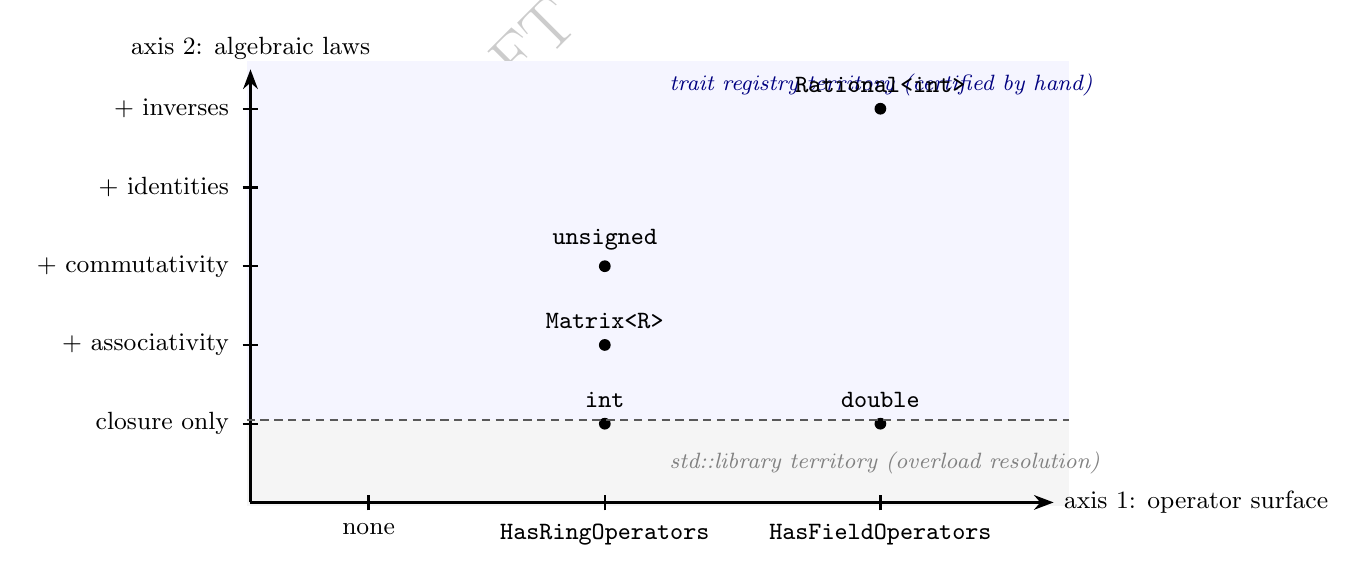
\begin{tikzpicture}[
  >={Stealth[length=2.5mm]},
  carrier/.style={circle, fill=black, inner sep=1.5pt},
  every node/.style={font=\small},
]
  % background bands
  \fill[gray!8] (-0.05,-0.05) rectangle (10.4,1.05);
  \fill[blue!4] (-0.05,1.05) rectangle (10.4,5.6);
  \node[anchor=west, font=\footnotesize\itshape, gray] at (5.2,0.5) {std::library territory (overload resolution)};
  \node[anchor=west, font=\footnotesize\itshape, blue!50!black] at (5.2,5.3) {trait registry territory (certified by hand)};

  % axes
  \draw[->, thick] (0,0) -- (10.2,0) node[anchor=west] {axis 1: operator surface};
  \draw[->, thick] (0,0) -- (0,5.5) node[anchor=south] {axis 2: algebraic laws};

  % horizontal ticks
  \foreach \x/\lbl in {1.5/{none}, 4.5/{\texttt{HasRingOperators}}, 8/{\texttt{HasFieldOperators}}} {
    \draw[thick] (\x,-0.1) -- (\x,0.1);
    \node[anchor=north] at (\x,-0.15) {\lbl};
  }

  % vertical ticks
  \foreach \y/\lbl in {1/{closure only}, 2/{+ associativity}, 3/{+ commutativity}, 4/{+ identities}, 5/{+ inverses}} {
    \draw[thick] (-0.1,\y) -- (0.1,\y);
    \node[anchor=east] at (-0.15,\y) {\lbl};
  }

  % carriers
  \node[carrier, label={[label distance=0pt]above:{\texttt{int}}}] at (4.5,1) {};
  \node[carrier, label={[label distance=0pt]above:{\texttt{unsigned}}}] at (4.5,3) {};
  \node[carrier, label={[label distance=0pt]above:{\texttt{double}}}] at (8,1) {};
  \node[carrier, label={[label distance=0pt]above:{\texttt{Rational<int>}}}] at (8,5) {};
  \node[carrier, label={[label distance=0pt]above:{\texttt{Matrix<R>}}}] at (4.5,2) {};

  % silence demarcation
  \draw[densely dashed, gray!70!black, thick] (-0.05,1.05) -- (10.4,1.05);
\end{tikzpicture}
\caption{\textbf{The two axes of the trait registry (draft).}  Axis 1 (horizontal) is the operator surface: which types compose under which operators.  This axis is validated by \emph{inspection} of the standard library --- overload resolution and concept binding answer it without further human input.  Axis 2 (vertical) is the algebraic-law stack: closure-only, then $+$ associativity, $+$ commutativity, $+$ identities, $+$ inverses.  Above the dashed line the standard library is silent: each law must be \emph{certified by hand}, per carrier, in the trait registry of §\ref{sec:algebraic_lattice_carriers}.  Carrier placements illustrate the typical shape of the silence: \texttt{int} closes the ring surface but signed-overflow UB defeats associativity (\textsc{ub}); \texttt{unsigned} reaches commutativity via modular arithmetic; \texttt{double} closes the field surface but IEEE-754 rounding defeats associativity; \texttt{Rational<int>} reaches the full field stack; matrix multiplication is associative without being commutative (a non-monotone point this stacked axis under-resolves --- see TODO note in source).  The placements are indicative; the audited data lives in the carrier rosettas (§\ref{sec:carrier-rosetta}).}
\label{fig:two-axes}
\end{figure}

The boundary of this architecture matches the core distinction in standard \Cpp{} between \emph{satisfying} a concept (syntactic structure) and \emph{modeling} it (semantic lawfulness).
Syntactic properties are mechanically decidable by the compiler.
Semantic properties---such as associativity or distributivity---resist mechanical verification inside standard \Cpp{} and remain the engineer's honesty obligation.
Here, $\mathbf{Jlt}$ defaults to an \emph{Honest Rejection Policy} which asserts that if neither mechanical nor manual certification is available at compile-time, then a violation of the corresponding axioms is assumed and the type is rejected at the gate.
For example, \texttt{int} satisfies the syntactic operators for a ring, but signed-overflow undefined behavior defeats associativity.
Conversely, \texttt{bool} is safely accepted as the Galois Field $\mathbb{F}_2$ because its bit-perfect operations never overflow or round, as demonstrated in Listing~\ref{lst:honest_rejection}.
This design mimicks the use of the \texttt{sorry} macro in Lean or the \texttt{Admitted} command in Coq, where a proof obligation is bypassed by fiat to allow downstream development.


By establishing this pure, disciplined substrate first, we gain an environment where types represent sets and values represent elements.
In category theory terms, we can write $\mathbf{Jlt} \subset \mathbf{Cpp}$.
This forms the exact Cartesian Closed Category needed to bootstrap formal set comprehension and universal algebra in the following sections.

\section{Intensional Sets as Type-Checked Predicates}
\label{sec:intensional_sets}

\begin{figure}[htbp]
\centering
\begin{tikzcd}[column sep=5em, row sep=4em, ampersand replacement=\&]
\mathbb{B} \arrow[loop above, "\neg"]
   \arrow[r, bend left=20, "\mathfrak{i}"]
\& \mathbb{N} \arrow[loop above, "x^2"]
   \arrow[l, bend left=20, "x \,\%\, 2 = 0"]
   \arrow[r, bend left=20, "-x"]
\& \mathbb{Z} \arrow[loop above, "-x"]
   \arrow[l, bend left=20, "x^2"]
\end{tikzcd}
\caption{
A sketch of the desired functionality to be supported by the \texttt{dedekind} set DSL.
The items shown correspond to a small example subset of $\mathbf{Alg}(\Sigma)$, the category of universal algebras.
Example canonical underlying carrier sets $\mathbb{B}$, $\mathbb{N}$, $\mathbb{Z}$ are shown as single objects, the individual set elements are omitted for brevity.
Most arrows on each carrier and most inter-carrier arrows are suppressed for clarity.
Selected endomorphisms are shown as loops: negation on $\mathbb B$, squaring on $\mathbb N$, negation on $\mathbb Z$.
Inter-carrier arrows are typed maps $\mathrm{T} \to \mathrm{S}$.
$\mathbb{B} \rightleftarrows \mathbb{N}$: forward $\mathfrak{i}$ the canonical embedding, reverse the parity classifier.
$\mathbb{N} \rightleftarrows \mathbb{Z}$: forward $x \mapsto -x$ (negation, well-typed as $\mathbb{N} \to \mathbb{Z}$ because $\mathbb{N}$ is not closed under additive inverse); reverse $x \mapsto x^2$ (squaring closes into $\mathbb{N}$ from any $\mathbb{Z}$ input).
The interested reader is referred to definitions of the category $\mathbf{FPL}$~\cite{pierce1991basic} which outlines similar steps in formal detail.
}
\label{fig:hub-spoke-bnz}
\end{figure}

With a deterministic, structurally-typed substrate established in Section~\ref{sec:jlt_posture}, mathematical sets can be bootstrapped inside the type system.
Here, we aim to model both the syntax and the semantics of mathematical set builder notation in executable $\mathbf{Jlt}$ hoping to achieve a system that lends itself to the expression and subsequent evaluation of precisely those kinds of problems that one might also encounter in a pure math blackboard setting.
A sketch of some desired supported functionality is provided in Figure~\ref{fig:hub-spoke-bnz}.

In this section, we first show working code (§\ref{sec:ddk_comprehension}) to illustrate the expected payoff, then discuss the theoretical foundations in set theory, specifically the category-theoretical elementary theory of sets (§\ref{sec:ddk_etcs}).

% ============================================================
\subsection{A Set Comprehension DSL}
\label{sec:ddk_comprehension}
% ============================================================

% Source: src/test/cpp/modules/dedekind/python/showcase_alpha_prime.cpp
\begin{listing}[htbp]
\caption{A code extract from the project's test suite intended to model set builder notation in C++23.
\cppinline{Set{...}} is a variadic constructor.
The combinators \cppinline{in} and \cppinline{bound} construct a scout variable and a half-space predicate respectively.
The scout variable appears on both sides of the bar: introduced on the left, and referred back to on the right, so the predicate to the right reads as the constraint $x > 5$.
\cppinline{operator()} is a shorthand for \cppinline{a.contains(e)}.
As evidenced by the \cppinline{static_assert}, the set operations are evaluated at compile time.}
\label{lst:pruning}
\begin{cpp}
// {x in ℕ | x > 5}
constexpr auto a = Set{in(ℕ) | in(ℕ) > bound<5>};
static_assert(a(7u) == a.contains(7u));

constexpr auto b = Set{in(ℕ) | in(ℕ) > bound<6>};
constexpr Singleton<6> c = a - b; 
constexpr auto d = Set{in(ℕ) | in(ℕ) < bound<7>};
constexpr Singleton<6> e = c & d;   
constexpr Ø<Cardinality> f = c & !c;                       

// {x in ℕ | ∃y ∈ e : x * y == 42}
constexpr Singleton<7> q = Set{in(ℕ) | Exists(e, [](auto y, auto x) { 
    return x * y == bound<42>; 
})};
\end{cpp}
\end{listing}

The combinator \cppinline{in} constructs a \emph{scout variable}.
In the blackboard form $\{\,x \in \mathbb{N} \mid P(x)\,\}$ it plays the role of the bound variable $x$: a stand-in for an arbitrary element of the domain, which the bar then constrains by a predicate.
What makes it more than a name is that it carries its domain in its own type, so the compiler knows what the variable ranges over.
Informally it just names an arbitrary element of that domain.
Formally it is the handle that the comprehension pipe (\cppinline{operator|}) binds to a predicate: in the code, \cppinline{BoundScout} is an empty structural type whose type-level ambient records the domain, gated by \cppinline{IsArrow} since a set is its own characteristic morphism.

This predicate-composition algebra is not merely a shorthand notation; it functions as an embedded syntax engine that allows the declaration of infinite spaces at the type level.
When operations like intersection (\texttt{\&}), union, or complement (\texttt{!}) are written as boolean logic combinations, the compiler parses the abstract syntax tree into a unified predicate chain.
The template engine expands these composed expressions during compilation, triggering type-level constant folding and dead-code elimination.

The correspondence is exact on the decidable track, and it is what makes the algebra optimizable.
Because a set is its predicate, the lattice of sets over a domain $A$ with decidable membership is the Boolean lattice lifted pointwise, $\mathcal{P}(A) \cong \mathbb{B}^A$ (Table~\ref{tab:lattice-lift}).
Where membership is undecided the codomain lifts to $\mathbb{B}+\text{U}$ and the operations become the three-valued Kleene ones, a de Morgan structure but no longer a Boolean algebra, since complement has no inverse at $\text{U}$.
Optimization is then the simplification of these predicate compositions at translation time: an empty meet prunes, $\bot \wedge p \Rightarrow \bot$, and constant conjuncts fold away.
The induced order, set inclusion, is pointwise implication $\chi_S \Rightarrow \chi_T$; it ranges over the domain, and keeping it decidable is the task of the specializations in §\ref{sec:ddk_etcs}.

\begin{table}[htbp]
\centering
\begin{tabular}{@{}lccccc@{}}
\toprule
lattice operation & meet & join & complement & bottom & top \\
\midrule
Boolean lattice $\mathbb{B}$ & $\wedge$ & $\vee$ & $\neg$ & $\bot$ & $\top$ \\
set lattice $\mathcal{P}(A)$ & $\cap$ & $\cup$ & $\complement$ & $\varnothing$ & $A$ \\
\bottomrule
\end{tabular}
\caption{
On the decidable track, the set lattice is the Boolean lattice, lifted pointwise.
An intensional set with decidable membership is its own total characteristic predicate $\chi : A \to \mathbb{B}$, so the powerset lattice over $A$ is the Boolean algebra of predicates, $\mathcal{P}(A) \cong \mathbb{B}^A$.
Each set operation is compiled as the corresponding Boolean operation on predicates, with no element materialized.
Undecidable membership lifts the codomain to $\mathbb{B}+\text{U}$, a three-valued Kleene structure that is not Boolean.
}
\label{tab:lattice-lift}
\end{table}

% Source: src/test/cpp/modules/dedekind/python/showcase_03_halfspace_contradiction.ll
\begin{listing}[htbp]
\caption{LLVM IR for the empty-meet witness in Listing~\ref{lst:pruning} (\texttt{clang++-22 -O2}): the membership query constant-folds to \texttt{ret i1 false}.}
\label{lst:pruning_ir}
\begin{cpp}
define noundef zeroext i1 @witness_empty_halfspace_meet() local_unnamed_addr #0 {
  ret i1 false
}
\end{cpp}
\end{listing}

The compiler is then allowed to perform aggressive compile-time verification and type-directed optimization.
When a membership test or set relation is encountered, the template engine expands the composed predicates and evaluates them during compilation.
If an intersection yields a logical contradiction, the type system reduces the resulting expression directly to the empty set $\emptyset$ before code generation occurs.
As a direct consequence, downstream runtime membership queries for statically impossible configurations are completely eliminated by the LLVM optimizer backend, collapsing into literal constant returns within the emitted machine instructions.
Listing~\ref{lst:pruning} exhibits a code base extract that tests this type-directed collapse in practice.
Listing~\ref{lst:pruning_ir} shows how this collapse is made mechanically observable during the build: the
witness function for set membership constant-folds to \texttt{ret i1 false} in the emitted LLVM IR.

% ============================================================
\subsection{Reifying A Category of Sets}
\label{sec:ddk_etcs}
% ============================================================

With the syntactic behavior of the set comprehension DSL established, what follows formalizes its semantic engine.
This intensional set layer is the disciplined fragment of §\ref{sec:jlt_posture} intersected with $\mathbf{Set}$, namely $\mathbf{Trsk} = \mathbf{Jlt} \cap \mathbf{Set}$: the Tarski layer where a set is a predicate and a graph is a relation, on which §\ref{sec:algebraic_lattice_carriers} imposes algebraic laws to reach $\mathbf{Ddk} = \mathbf{Trsk} \cap \mathbf{Alg}$.
Loosely speaking, a set here is just its membership test.
A reader who wants only the API can keep that picture and skim the rest of this subsection, which makes it precise in the language of topos theory.
The more common description of sets, the one \cppinline{std::set} follows, is Zermelo-Fraenkel (ZF): a set is built from the bottom up from atoms such as $\emptyset$ via union and intersection, with membership tested by an element relation ($\in$).
Its obvious reading is a bag with things in it, and an implementation stores exactly that, the elements in memory, so it is \emph{extensional} by definition.
That reading does not fit every set one wants to compute with.
Take the open disk $D = \{\, x \mid \lVert x - c \rVert < r \,\}$ in the plane: extensionally a bag of uncountably many points that no machine can hold, intensionally a single inequality that \emph{is} the set.
This is the everyday contrast between a raster image and a vector drawing: extensionally the disk is a grid of stored points, intensionally it is the defining inequality, exact at any resolution.
% FIXME(restructure): candidate wrapfigure. Side-by-side rendering of the same
% disk: left a raster / pixel grid (extensional / ZFC, the stored points), right a
% vector drawing labelled by the predicate (intensional / ETCS, the defining
% condition). Caption: raster-vs-vector = extensional-vs-intensional = ZFC-by-
% contents vs ETCS-by-condition. Alt design: a Venn whose overlap P and Q ties to
% the lattice-lift table (intersection IS conjunction). Keep it small; decide at
% the 22pp main/appendix split.
ETCS gives a natural language for this second perspective, where a set is presented by the condition its members satisfy, a perspective the bag-of-things reading of ZF leaves implicit.

To escape the limitations of resource-bounded containers, \texttt{dedekind} shifts from an extensional formulation to a structural, category-theoretic foundation.
The library acts as a change-of-base engine across a diagram of distinct structural set theories.
What it guarantees for any predicate is a correct general default, and that default is deliberately poor.
Hand the engine an opaque C++ lambda and it is honest but unoptimized.
By Rice's theorem~\cite{rice1953classes} the compiler cannot inspect a black-box function to prune a meet or reduce an active set at translation time.
A point query still runs the lambda.
A structural query the compiler cannot search, such as emptiness or an existential over an unbounded domain, returns a deterministic \texttt{Unknown} rather than risking a translation-time hang.
So the default gives one of three answers: yes, no, or \texttt{Unknown}, the last meaning only that the test did not finish at compile time.
The open disk shows the shape of it: inside tests yes, outside tests no, and the rim $\lVert x - c \rVert = r$ is where a decision can stall.
An ordinary floating-point comparison still returns a definite bool there; the rim is genuinely \texttt{Unknown} only for a carrier that reports the undecided boundary rather than forcing $<$ or $=$, the role \texttt{dedekind}'s constructive $\mathbb{R}$ is meant to play.
That third answer is not a new kind of truth; it records that the query was left undecided.
Formally, yes and no stay the ordinary two-valued truth object ($\Omega = \mathbb{B}$), and \texttt{Unknown} is a separate value layered on top: the \emph{lift} of the Booleans, or partial-map classifier~\cite{moggi1991notions, rosolini1986continuity}.

Optimization is opt-in, through specialization.
The type system exposes a family of named, structurally transparent predicates that specialize for a selection of common classifications: extensional sets, partially ordered sets, totally ordered sets, and so on.
When a carrier matches one, the compiler reads its structure, fires the rewrite rules of Theorem~\ref{thm:type-directed-collapse-1d}, prunes at compile time, and decides membership.
The answer is then always a plain yes or no, the two-valued logic every programmer expects ($\Omega = \mathbb{B}$).
The shared set interface (\cppinline{IsSet}) presents both paths identically to the downstream code, so a specialization is a drop-in fast path, not a separate type.
% IMPLEMENTATION NOTE (2026-08-17, spec vs code): this sentence and
% Figure~\ref{fig:compiler_decision_tree}'s "none -> B+U" branch state the SPEC.
% The current resolver only approximates it: NaturalLogic keys on IsCountable
% (a cardinality proxy, unsound for an opaque predicate over a countable domain)
% plus structural reductions, NOT on decidability. An opaque bool lambda always
% yields a definite value via lift_logic, never Unknown. Target: make
% HasDecidableMembership the primary gate (IsExtensional OR a structural-
% decidability witness advertised by the named predicate) and derive
% logic_species from it. Tracked as a follow-up code PR; blast radius ~239 test
% references to ClassicalLogic / NaturalLogic. See PR #766 review discussion.
The split is therefore not by cardinality but by whether a specialization applies.
The catalogue of structured presentations, and the algebra of which set operations preserve the fast path, is the subject of §\ref{sec:algebraic_lattice_carriers}.

\begin{figure}[htbp]
\centering
\begin{tikzcd}[row sep=1.8em, column sep=2.6em, ampersand replacement=\&]
\& \& \& \mathbb{B} \arrow[r, "\chi"] \& \{\top, \bot\} \\
T \arrow[r, "\text{inspect}"] \& \mathbf{Jlt} \arrow[r, "\text{yes}"] \arrow[d, "\text{no}"'] \& |[draw, rounded corners]| \text{specialization?} \arrow[ur, "\text{matches}"] \arrow[dr, "\text{none}"'] \& \& \\
\& \text{Reject} \& \& \mathbb{B}+\text{U} \arrow[r, "\chi"] \& \{\top, \bot, \text{U}\}
\end{tikzcd}
\caption{
The one decision the semantic engine makes on type inspection.
Carriers failing the $\mathbf{Jlt}$ gate (non-\texttt{std::regular}) are rejected by concept constraints.
Rice's theorem rules out a universal fast path, so the library ships a correct general default and lets the user opt into optimization by specializing.
When a carrier matches a named, transparent presentation, the compiler reads its structure, prunes at compile time, and decides: membership is two-valued and the classifier is Boolean, $\Omega = \mathbb{B}$.
When none matches, only the opaque predicate remains, and a query the compiler cannot search returns a deterministic \texttt{Unknown} rather than risking a translation-time hang.
That default is a partial characteristic map into the lifted Boolean $\mathbb{B}+\text{U}$, where \texttt{U} records definedness, not a third truth.
}
\label{fig:compiler_decision_tree}
\end{figure}

When one side of an \texttt{and} or \texttt{or} is \texttt{Unknown}, the result follows the rule you would hope for.
An intersection with a provably empty set is still empty even if the other side is undecided ($\bot \wedge \text{U} = \bot$), so the prune survives.
This is exactly what compile-time pruning needs, and it is stronger than threading the unknowns through a \texttt{Maybe}-style combinator, which would surrender and return \texttt{Unknown} the moment either side is unknown, losing the prune.
Formally these are the strong-Kleene, or \emph{parallel}, connectives, and the resulting three-valued logic of partial predicates is Kleene's, not an intuitionistic one: the underlying truth values stay Boolean, and the third value marks undecidedness~\cite{kleene1952metamathematics, plotkin1977lcf}.
The upshot is that a query the compiler cannot enumerate returns a definite \texttt{Unknown} during translation rather than hanging, and the structural guarantees survive intact.
Figure~\ref{fig:compiler_decision_tree} shows the decision.

\begin{listing}[ht]
\caption{
Excerpts from \texttt{dedekind} illustrating the \cppinline{concept} definitions used in the reification of $\mathbf {Ddk} \subseteq (\mathbf{Set} \cap \mathbf{Jlt})$.
Fundamental \cppinline{concept} definitions (objects, morphisms, small categories, \ldots) are composed to reify the considerably more complex \cppinline{concept IsSet}.
\cppinline{concept IsSet} can then be used to mechanically test candidate implementations of set theory in the ETCS sense.
Left: definition of morphisms and small categories: \cppinline{concept IsArrow}, \cppinline{IsMonicArrow}, \cppinline{IsEpicArrow}, \cppinline{IsIsomorphism}, \cppinline{IsSmallCategory}.
Right: the characteristic-map axiom \cppinline{IsSubobject}, where a subobject's own call shape \cppinline{s(a)} is the classifier $\chi : A \to \Omega$ (it returns a \cppinline{LogicalValue}); and the composite \cppinline{IsSet}, a \cppinline{Jlt} carrier that conjoins the ten ETCS axiom witnesses (\cppinline{HasETCSAxioms}) with the Set-as-Cartesian-closed-category witness.
The interested reader is referred to the reference implementation~\cite{Krautler_dedekind_2026} for full implementation details.
}
\label{lst:concept_isset}
\noindent
\begin{minipage}[t]{0.48\linewidth}
$\mathbf{Cat}$ in $\mathbf{Jlt}$
\begin{cpp}
export template <typename F>
concept IsArrow = requires {
  typename std::remove_cvref_t<F>::Domain;
  typename std::remove_cvref_t<F>::Codomain;
} && requires(F f, typename std::remove_cvref_t<F>::Domain x) {
  { f(x) } -> std::convertible_to<typename std::remove_cvref_t<F>::Codomain>;
};
\end{cpp}
\end{minipage}\hfill
\begin{minipage}[t]{0.48\linewidth}
$\mathbf{Set}$ in $\mathbf{Jlt}$
\begin{cpp}
template <typename S, typename A>
concept IsSubobject = requires(S s, typename S::Member m, A a) {
  { s.ι(m) } -> std::same_as<A>;
  { s(a) }   -> LogicalValue;
};

template <typename A>
concept IsSet =
  HasETCSAxioms<A> &&
  IsCartesianClosed<CanonicalSetCCC<typename A::Ambient>>;
\end{cpp}
\end{minipage}
\end{listing}

The semantic engine above presupposes a categorical, rather than extensional, notion of set.
That notion is Lawvere's~\cite{lawvere1964etcs}: a set is given \emph{intensionally}, by objects and the functions (morphisms) between them.
Here, we use the following literature definition~\cite{nlab:nlab}: \emph{$\mathbf{Set}$ is a \textbf{well-pointed}, \textbf{Cartesian Closed Category} with a \textbf{subobject classifier}, a \textbf{natural numbers object}, and the \textbf{axiom of choice}}.
This definition is arguably terse and full of jargon, but it can be broken down into 10 defining axioms.
These axioms can in turn be reified as type-level \cppinline{concept} predicates and composed into an overall structural type predicate \cppinline{concept IsSet} which can then be used to check if a type in $\mathbf{Jlt}$ is also an object in $\mathbf{Set}$.
The interested reader is referred to  Mac Lane~\cite{maclane1971categories} for an in-depth treatment and to Pierce~\cite{pierce1991basic} for a pedagogical introduction to many of the key concepts.

Here, we present a reification of its 10 defining axioms in terms of a type-predicate (\cppinline{concept IsSet}) reified in $\mathbf{Jlt}$.
The implementation is layered into a number of steps, each step refining the \cppinline{concept} in question and introducing applicable terminology from category theory and set theory respectively so that readers familiar with any of these schools should be able to follow.
For the sake of brevity, the steps are detailed in Appendix~\ref{sec:etcs}, key excerpts from the code base are summarized in Listing~\ref{lst:concept_isset}.

A concrete type that type checks against \cppinline{concept IsSet} should support all of the above functionality and allow the evaluation of non-trivial set expressions as one might encounter them in a blackboard environment.

Identity is denoted by an identity arrow, and set membership is tested by evaluating a predicate on a value.
The steps taken to reify intensional sets in the code base form a core category $\mathbf{Ddk} \subset \mathbf{Jlt} \cap \mathbf{Set}$, which occupies the intersection of pure $\mathbf{Jlt}$ types and universal-algebraic set structures.
The implementation tracks this definition literally at compile time.

First-order quantification is restricted to domains satisfying \cppinline{IsExtensional}, as unconstrained evaluation over infinite intensional spaces is undecidable at compile time.
For these bounded domains, the quantifiers $\exists$ (\cppinline{Exists}) and $\forall$ (\cppinline{ForAll}) map directly onto finite coordinate-wise reductions ($\bigvee$ and $\bigwedge$) over $\Omega$, executing as zero-overhead variadic fold expansions during template translation.

\section{Point-Free Mappings: Functors between Sets}
\label{sec:relations_functions_blueprint}

To transition seamlessly from static intensional sets to dynamic mappings, binary relations can be formalized as morphisms \cppinline{IsArrow<A, B>} where both domain and codomain \cppinline{require} the ETCS axioms via \cppinline{IsSet}. 
Such morphisms are then classified by the following properties, if one focuses on the domain:
\begin{itemize}
    \item \textbf{Totality}: Outgoing arrows per input $\ge 1$.
    \item \textbf{Functionality}: Outgoing arrows per input $\le 1$.
    \end{itemize}
 And if one focuses on the codomain:
 \begin{itemize}
    \item \textbf{Injectivity}: Incoming arrows per output $\le 1$.
    \item \textbf{Surjectivity}: Incoming arrows per output $\ge 1$.
\end{itemize}
Equivalently, relations can be represented as sets whose elements satisfy the product axioms (\cppinline{IsProduct}), for example via the signature \cppinline{IsSet<std::pair>}.

\begin{listing}[htbp]
\caption{Intensional specification of a binary relation predicate over an algebraic product space and its pointwise validation.}
\label{lst:intensional_relation_validation}
\begin{cpp}
// R = { (a, b) ∈ ℕ × ℕ | b % a == 0 }
constexpr auto x = var(ℕ * ℕ);
constexpr auto R = Set{
    x | (π_2(x) % π_1(x) == bound<0>)
};

// Pure pointwise validation via indicator properties
static_assert(R(std::pair{2u, 6u})); // Validated: 6 % 2 == 0
static_assert(!R(std::pair{4u, 6u})); // Rejected: 6 % 4 != 0
\end{cpp}
\end{listing}

The design of the relation $R$ in Listing~\ref{lst:intensional_relation_validation} highlights the core architectural boundary between symbolic specification and type-level evaluation.
Structurally, the relation is defined entirely through an intensional presentation.
Rather than relying on explicit, verbose template-parameter bindings, the expression leverages the functional factory \texttt{var(}\dots\texttt{)} to inject a value-level token carrying the underlying product domain mechanics of $(\mathbb{N} \times \mathbb{N})$.
This variable placeholder binds the relational invariant as a native type-directed predicate. 

This intensional rule collapses into an extensional, pointwise evaluation context when interrogated by a concrete element via the indicator property \texttt{operator()}.
During compilation, the \texttt{static\_assert} forces the template engine to substitute the candidate literal pair into the projection bindings $\pi_1$ and $\pi_2$, reducing the symbolic constraint down to a primitive boolean literal.
Consequently, the library maintains the abstract economy of mathematical logic right up until specific domain elements witness the correctness of the constraint at compile time.

In classical relational calculus, the relative composition of two relations $R \subseteq A \times B$ and $S \subseteq B \times C$ requires an existential quantification step over the intermediate domain $B$:
\begin{equation}
R \circ S = \{ (a, c) \in A \times C \mid \exists b \in B : (a, b) \in R \land (b, c) \in S \}
\end{equation}
However, general first-order existential ($\exists$) and universal ($\forall$) quantification cannot be implemented generically over infinite intensional sets at compile time, as the enumeration of open predicate domains induces infinite compiler loop regression. 

To circumvent this translation-time decidability bottleneck, the library rejects identifying a relation extensionally as a static subobject pair $R \subseteq A \times B$. Instead, it implements a monadic presentation where a relation is an active functional morphism. Concretely, a binary relation $R$ from a domain set $A$ to a codomain set $B$ is defined as a total arrow of the form $R : A \to \mathcal{P}(B)$, where $\mathcal{P}(B)$ represents the intensional power set of the target space. This architectural choice ensures that when an element $a \in A$ is supplied to the relation, the compiler immediately evaluates the image as a native, optimized intensional set type in the destination space.

Under this functional presentation, Tarski's relative composition resolves elegantly as standard Kleisli arrow composition over the power set monad. We explicitly reify this step within the \texttt{:relations} partition via the infix pipeline operator ($\gg$), allowing the point-free composition to be expressed textually as:
\begin{equation}
R \mathbin{\gg} S : A \to \mathcal{P}(C)
\end{equation}
The template engine executes this composition by mapping $R$ over an input element to yield an intermediate set, and then binding $S$ across that resulting image via an intensional set-theoretic union cascade:
\begin{equation}
(R \mathbin{\gg} S)(a) = \bigcup_{b \in R(a)} S(b)
\end{equation}

\begin{listing}[htbp]
\caption{Point-free relational composition via Kleisli arrow piping over the power set monad, circumventing explicit existential quantification search bounds.}
\label{lst:kleisli_fish_composition}
\begin{cpp}
// R : ℕ → P(ℕ) where R(a) = { b ∈ ℕ | b % a == 0 }
constexpr auto R = [](auto a) {
    constexpr auto b = var(ℕ);
    return Set{ b | (b % a == bound<0u>) };
};
// S : ℕ → P(ℕ) where S(b) = { c ∈ ℕ | b < c }
constexpr auto S = [](auto b) {
    constexpr auto c = var(ℕ);
    return Set{ c | (b < c) };
};
// Point-free Tarskian relative composition via the fish operator
constexpr auto R_then_S = R >> S;
// Pointwise validation: The compiler lazy-chains the predicates
// Is 5 in the composition image of 2? Validated: 
static_assert((R_then_S(2u))(5u));
// Is 3 in the composition image of 4? Rejected.
static_assert(!(R_then_S(4u))(3u));
\end{cpp}
\end{listing}

Because the underlying power set operations evaluate purely as compile-time predicate transformations, the composition of two relations does not trigger a runtime search loop over the intermediate space.
The infix pipeline operator ($\gg$) implements true Kleisli composition; when evaluated at a point $a$, the template engine skips any raw search loop and instead transforms the symbolic predicate of $R$ directly into the input of $S$.
The existential requirement is thus safely re-encoded as a lazy, zero-cost symbolic predicate transformation pipeline. 

The compiler unifies the constituent predicates into a single, synthesized type-level constraint that governs the end-to-end mapping from $A$ to $C$. Listing~\ref{lst:kleisli_fish_composition} illustrates how this monadic relation concept and its corresponding Kleisli composition operator are structurally declared inside the toolchain.

\subsection{Functions and Morphism Factorization Gates}
\label{sec:functions_morphism_factorization}

While the relational composition operator ($\gg$) detailed in Section~\ref{sec:relations_functions_blueprint} bypasses the need for intermediate set materialization by maintaining a lazy symbolic predicate chain, specialized functional mappings impose a more stringent computational burden.
For total functions where elements must be explicitly mapped and verified as certified singleton images, the template engine cannot rely solely on passive predicate encapsulation.
If a function lacks a strict structural inverse or is evaluated over an unconstrained, transfinite domain, constructively determining image containment or mapping preimages becomes undecidable at translation time. Consequently, if a generic result-set construction is impossible for general functions, it is similarly precluded for general relations.
To resolve this boundary, the library introduces an architectural gate based on the categorical principle of epic-monic factorization.

Mathematically, a relation $R : A \to \mathcal{P}(B)$ is identified as a total function if and only if it maps every input element $a \in A$ to a certified singleton subset in the codomain.
In the codebase, this structural guarantee is enforced within the \texttt{:functions} partition by wrapping the underlying relation inside a specialized function adapter and guarding its evaluation site with an \texttt{IsSingleton} concept constraint.
This architecture preserves the structural continuity of the library: functions are not distinct primitives, but are well-behaved, deterministic relations whose output logic is structurally bounded.

Reifying functions in this manner allows the type system to mechanically verify classical mapping properties at translation time.
For specialized mappings, codomain membership tests, checking whether a given element $b \in B$ lies within the actual image of the transformation, are easily discharged by the compiler.
If a function is certified as surjective, every element of the target space is a valid image, meaning a codomain membership query trivially constant-folds to logical truth.
If a function is bijective, as is already implemented and leveraged within the core set eDSL, the type system utilizes a structural left-and-right inverse witness to map elements bi-directionally between spaces with zero runtime overhead.

\begin{listing}[htbp]
\caption{Intensional specification of a functional range via analytical inversion of a bijective function.}
\label{lst:functional_image_bijection}
\begin{cpp}
// Bijective case: { n + 2 ∈ ℕ }
constexpr HalfSpace<2> p2 = Set{in(ℕ) + bound<2u>}; 
static_assert(!p2(0));
static_assert(p2(3));
\end{cpp}
\end{listing}

For general or non-bijective functions, however, validating whether an arbitrary element $b \in B$ possesses a valid preimage in the domain $A$ presents a severe decidability barrier if evaluated via standard search techniques.
Rather than treating this as an impassable restriction, the library provides specialized support for functional relations by introducing an architectural gate based on the categorical principle of epic-monic factorization.
Every general functional arrow $f : A \to B$ can be factored into a regular surjection (epi) onto an intermediate image set $I$, followed by a regular injection (mono) from $I$ into the destination space $B$:
\begin{equation}
A \twoheadrightarrow I \hookrightarrow B.
\end{equation}

By requiring the developer to provide this factorization mapping when declaring an arbitrary \cppinline{IsTotalFunction}, the compiler gains the exact structural properties needed to handle general codomain membership tests.
Since the second leg of the factorization chain is a strict injection, it guarantees a one-to-one mapping from the intermediate image set $I$ into the target space $B$, allowing the type-checker to reason about the embedding without exploring the raw domain space $A$.
Listing~\ref{lst:functional_image_factorization} illustrates how this epic-monic gate and its corresponding image validation assertions are codified within the C++23 template engine.

\begin{listing}[htbp]
\caption{Intensional specification of a functional image set via forward epic-monic composition inside a set comprehension block, followed by an intensional \cppinline{max} collapse to a value singleton.}
\label{lst:functional_image_factorization}
\begin{cpp}
constexpr auto x = var(ℕ);
// Non-bijective case via explicit factorization:
// { x * x ∈ ℕ | x < 5 }
// The left-hand side pipes the epi leg into the mono gate via operator>>
constexpr auto sqs = Set{ 
    (x * x) >> is_square | x < bound<5u> 
};

// An intensional max reduction extracts the peak element from the image set
constexpr Singleton<16u> max_square = max(sqs);
\end{cpp}
\end{listing}

By utilizing the \texttt{mono\_retract} partial witness, the compiler can evaluate codomain properties purely as a local lookup on the intermediate type boundary.
This structural approach ensures that even highly complex or non-linear functional images can be safely validated at compile time.
The type system can consequently treat arbitrary transformations as well-behaved objects, laying a reliable foundation for the universal algebraic operators and endofunction loops developed in the subsequent section.

%------
\section{Universal Algebra and the Algebraic Lattice of Carriers}
\label{sec:algebraic_lattice_carriers}
%-------

% Source excerpt from dedekind.algebra:universal.
\begin{listing}[ht]
\caption{A type that type-checks against \cppinline{IsAlgebraOnSet} inhabits $\mathbf{Ddk}$.}
\label{lst:algebra:universal}
\begin{cpp}
export template <typename X, typename... Ops>
concept IsAlgebraOnSet =
    IsSet<X>                                          // Trsk: X is a set
    && (... && IsClosedUnderEither<X::Domain, Ops>)   // closure: each op corresponds to endomorphisms
    && IsAlgebra<X::Domain, Ops...>;                  // the (A, F) algebra
\end{cpp}
\end{listing}
A carrier in \texttt{dedekind} is an \emph{algebraic set}: a C++ type that is a set in the sense of §\ref{sec:intensional_sets} and carries operations on that set.
A type inhabits the category $\mathbf{Ddk}$ exactly when it type-checks against \cppinline{IsAlgebraOnSet} (Listing~\ref{lst:algebra:universal}), which asks for both halves at once: that the type is a set (the Tarski layer $\mathbf{Trsk}$ of §\ref{sec:intensional_sets}) and that its carrier is closed under the operations it supplies:
\begin{equation}
    \mathbf{Ddk} \;=\; \mathbf{Trsk} \,\cap\, \mathbf{Alg}(-),
\end{equation}
the algebraic sets expressible as C++ types.
Because membership is structural, admission is after the fact: a type is presented as a set by a concept, with no change to the type and no upstream opt-in.

Figure~\ref{fig:hub-spoke-bnz} is a sketch of this category, and it is worth keeping in hand for the rest of the section.
Its objects are algebraic sets, the hubs $\mathbb{B}, \mathbb{N}, \mathbb{Z}$, drawn with a few representative arrows and the rest suppressed.
The loops are endomorphisms of a carrier: negation on $\mathbb{B}$, squaring on $\mathbb{N}$, negation on $\mathbb{Z}$.
The arrows between hubs are typed maps $\mathrm{T} \to \mathrm{S}$: the canonical embedding $\mathbb{B} \hookrightarrow \mathbb{N}$ with the parity classifier back, and $x \mapsto -x$ from $\mathbb{N}$ into $\mathbb{Z}$ (well-typed precisely because $\mathbb{N}$ has no additive inverse) with squaring back.
Reading a hub as a bare carrier, forgetting its operations, is the forgetful functor $U : \mathbf{Alg}(-) \to \mathbf{Set}$, and a plain set is the degenerate hub whose loop is empty.
$\mathbf{Alg}(-)$ is universal algebra in the textbook sense~\cite{burris1981universalalgebra}: sets equipped with operations of fixed arity, where the dash is a placeholder for whatever signature a carrier happens to supply.\footnote{We leave the signature unbound and let the per-shape \cppinline{Has*Operators} concepts pin it at each carrier's definition, so $\mathbf{Ddk}$ stays as wide as the library needs while a concrete variety such as $\mathbf{Mon}$ or $\mathbf{Ring}$ is one fixed choice of dash (the same $F_\Sigma$-algebra fragment a functional programmer would recognise~\cite{pierce1991basic}).  We also fix a smallness ceiling of $\beth_1$, carriers no larger than the continuum, which is enough for $\mathbb{R}$, $\mathbb{C}$, and $\mathbb{D}$ while keeping the encoding clear of the proper-class self-reference that $\mathbf{Set}$ and $\mathbf{Cat}$ court; the meta-categorical bookkeeping this defers (size-hierarchy adjunctions, $\mathrm{Disc} \dashv U$) survives as the engineer's honesty obligation, treated in the companion report.  The simply-typed-$\lambda$-calculus and System~F reading of the same fragment is Appendix~\ref{app:jlt-systemf}.}

The smallest inhabitant makes the shape concrete.
The Boolean carrier $\mathbb{B}$ is an algebraic set the moment it type-checks as $\mathbf{Alg}(\wedge, \vee, \neg)$ over \cppinline{bool} (Listing~\ref{lst:algebra:boolean_case}): the object is the set, the three operators are its self-loops.

% Source excerpt from dedekind.algebra:boolean.
\begin{listing}[ht]
\caption{Case Study: \cppinline{𝔹} is a bit-perfect algebraic set in $\mathbf{Ddk}$ by way of inhabiting $\mathbf{Jlt}$ as well as $\mathbf{Alg}(∧, ∨, ¬)$.}
\label{lst:algebra:boolean_case}
\begin{cpp}
export inline constexpr UniversalSet<bool, ClassicalLogic, Finite> 𝔹 =
    sets::Ω<bool>;

static_assert(
    IsAlgebraOnSet<decltype(𝔹),             // X = decltype(𝔹) —
                                            // the SET
                   std::logical_and<bool>,  // ∧  ┐
                   std::logical_or<bool>,   // ∨  ├ F = element-level ops
                   std::logical_not<bool>   // ¬  ┘   on the carrier bool
                   >);
\end{cpp}
\end{listing}

\subsection{The carrier lattice}
\label{sec:carrier-lattice}

The carriers form a lattice, and the library builds it the way the textbooks do, one universal-property construction at a time.
The bottom is the Boolean semiring $\mathbb{B}$ above, with the naturals $\mathbb{N}$ just over it.
From there the tower is the standard one: the Grothendieck completion of $(\mathbb{N}, +)$ to the integers $\mathbb{Z}$ and their field of fractions $\mathbb{Q} = \operatorname{Frac}(\mathbb{Z})$, Dedekind cuts to the reals $\mathbb{R}$, free modules to the vector and matrix carriers $R^n$ and $M_n(R)$, and polynomial quotients to the complex and dual numbers, $\mathbb{C} = \mathbb{R}[i]/(i^2{+}1)$ and $\mathbb{D} = \mathbb{R}[\varepsilon]/(\varepsilon^2)$.
None of this is ours to reprove: it is Bourbaki's structuralist tower~\cite{bourbaki1968theoryofsets, marquis2022structuralist} carried down to the type level, and the textbooks treat it better than we could.
The only discipline the library adds is that each rung lifts at the type level the moment a hub naming it passes its concept gate, so it is the compiler, not the reader, that checks each construction is what it claims to be.

The quotient rung is backed by the First Isomorphism Theorem, $A/\ker f \cong \operatorname{im} f$~\cite{burris1981universalalgebra}, which \texttt{category:image} records as a typed claim: the quotient and image are registered per homomorphism, and a supplied isomorphism is type-checked against them.

\subsection{Certified laws travel with the carrier}
\label{sec:hsp_varieties}

What makes these carriers usable downstream is that their \emph{laws} propagate.
A class of algebras closed under homomorphic images, subalgebras, and products is a variety (Birkhoff~\cite{burris1981universalalgebra}), and the library realises that closure as \emph{trait propagation}: when a carrier is derived by an H, S, or P construction, the species traits it satisfies (\cppinline{is_associative_v}, \cppinline{is_commutative_v}, \cppinline{is_distributive_v}, and the rest) propagate to the derived carrier, confirmed there by \cppinline{static_assert}.
Listing~\ref{lst:hsp-closed} pins this at the cyclic base $\mathbb{Z}/6\mathbb{Z}$: the variety ``associative and commutative $+$'' stays closed across its H, S, and P images, witnessed by eight \cppinline{static_assert}s.
The gate §\ref{sec:optimization_lp} uses, \cppinline{IsSemiring}, reads this same species-trait registry; the tropical carrier registers its own entries directly rather than as an H, S, or P image, so the exhibit's gate is a registry lookup, not a re-proof.

\begin{listing}[ht]
\caption{Birkhoff's HSP closure typed.  Base $\mathbb{Z}/6\mathbb{Z}$ + three synthetic HSP markers wired to the carrier-side registries; the trait propagation lifts both axioms of the variety uniformly to all three HSP-derived carriers.  Any future H/S/P construction over $\mathbb{Z}/6\mathbb{Z}$ (or any other base in the variety) follows the same one-line opt-in pattern.}
\label{lst:hsp-closed}
\begin{cpp}
// --- Synthetic HSP markers wired to Modular<6> -----------------------
struct H_image_of_Z6 {};   // type-level placeholder for any H-image of Z/6Z
struct S_subalg_of_Z6 {};  // ... S-subalgebra ...
struct P_product_of_Z6 {}; // ... P-direct-product ...

template <> struct quotient_algebra_base<H_image_of_Z6> { using type = Modular<6>; };
template <> struct subalgebra_base      <S_subalg_of_Z6> { using type = Modular<6>; };
template <> struct product_algebra_base <P_product_of_Z6>{ using type = Modular<6>; };

// --- THE Birkhoff HSP-closed crown -----------------------------------
// Variety V: carriers with associative + AND commutative +.
// V is HSP-closed by the propagation specs.

using Z6 = Modular<6>;  using H = H_image_of_Z6;
using S  = S_subalg_of_Z6;  using P = P_product_of_Z6;

static_assert(is_associative_v<Z6, std::plus<Z6>>);  // base ∈ V
static_assert(is_associative_v<H,  std::plus<H>>);   // H closure (quotient)
static_assert(is_associative_v<S,  std::plus<S>>);   // S closure (subalgebra)
static_assert(is_associative_v<P,  std::plus<P>>);   // P closure (product)
static_assert(is_commutative_v<Z6, std::plus<Z6>>);  // (same four, both axioms)
static_assert(is_commutative_v<H,  std::plus<H>>);
static_assert(is_commutative_v<S,  std::plus<S>>);
static_assert(is_commutative_v<P,  std::plus<P>>);
\end{cpp}
\end{listing}


\subsection{Dual numbers, for the sensitivity exhibit}
\label{sec:dual_numbers_quotient}

The one carrier worth a second look, because §\ref{sec:optimization_lp} differentiates with it, is the dual numbers, mathematically the quotient ring $\mathbb{D} = \mathbb{R}[\varepsilon]/(\varepsilon^2)$.
The implementation is that quotient's direct realisation: a pair $(a, b)$ whose multiplication is written as $(a, b)(c, d) = (ac,\, ad + bc)$, with the truncation $\varepsilon^2 = 0$ already discharged in the formula.
The operator is \cppinline{constexpr}, so a product of compile-time operands folds during translation, and the $\varepsilon$-coordinate carries the derivative: forward-mode automatic differentiation as a ring law (Listing~\ref{lst:lin-alg-embeddings}).

% Source: src/test/cpp/modules/dedekind/linear_algebra/embeddings_test.cpp
\begin{listing}[htbp]
\caption{Dual numbers embed faithfully as $2 \times 2$ matrices over $\mathbb{Q}$, with the infinitesimal squaring to zero.}
\label{lst:lin-alg-embeddings}
\begin{cpp}
using Rat = Rational<SignedExtensionalCardinal<>>;
constexpr Dual<Rat> d{Rat{2}, Rat{3}}, e{Rat{-1}, Rat{5}};
static_assert(as_matrix2x2(d + e) == as_matrix2x2(d) + as_matrix2x2(e));
static_assert(as_matrix2x2(d * e) == as_matrix2x2(d) * as_matrix2x2(e));
constexpr Dual<Rat> eps{Rat{0}, Rat{1}};
static_assert(as_matrix2x2(eps) * as_matrix2x2(eps) == zero_matrix2x2_v<Rat>);
\end{cpp}
\end{listing}

\section{Coordinate-Free Operators: Boundary and Coboundary}
\label{sec:operational_calculus}
\label{sec:geometric_mappings}

With the carriers of §\ref{sec:algebraic_lattice_carriers} in place, the linear algebra over them stays coordinate-free.
A linear map is not stored as a grid of coefficients and walked by index; the two operators a graph actually needs are kept as structural, matrix-free mappings between functions on its cells.
A graph is a one-dimensional complex: a node potential is a 0-form $d : \mathcal{V} \to S$, an edge value a 1-form on $\mathcal{E}$.

The \emph{coboundary} $\delta$ is the discrete gradient, sending a node 0-form to the edge 1-form of its differences,
\begin{equation}
    (\delta d)(u \to v) = d(v) - d(u),
\end{equation}
and the \emph{boundary} $\partial$ is its adjoint, sending a directed chain to its signed endpoints, $\partial[\,s \to t\,] = \{t\} - \{s\}$.
Neither is materialised; each is an expression over the incidence structure.
The mnemonic is calculus: $\delta$ is the differential (a difference of potentials), $\partial$ is evaluation at the endpoints, and the discrete Stokes theorem $\int_\gamma \delta d = \langle d,\ \partial\gamma\rangle$ ties them.

These two operators are what pose the problem §\ref{sec:optimization_lp} solves.
The critical-path duration is the boundary pairing $\langle d,\ \partial\gamma\rangle = d(t) - d(s)$, and the precedence constraints are the coboundary bound $\delta d \ge c$, so the dual program is
\begin{equation}
    \text{minimise}\ \langle d,\ \partial\gamma\rangle \quad\text{s.t.}\quad \delta d \ge c .
\end{equation}
Section~\ref{sec:optimization_lp} is that program's solver in the tropical semiring: its closure is the integral that inverts $\delta$, accumulating cost along paths to recover $d$ (realised as a fold, not a reified operator).
So this section is not adjacent to the exhibit; it supplies the operators the exhibit is written in.

\section{Optimization by Semiring Closure}
\label{sec:optimization_lp}

We turn from the set primitives to a high-utility application, and the step is a short one, because a graph is already a relation.
A directed graph on a node set $\mathcal{V}$ is a relation $E \subseteq \mathcal{V} \times \mathcal{V}$, which the comprehension DSL of §\ref{sec:ddk_comprehension} expresses \emph{intensionally}, as a predicate on a pair of nodes rather than as a stored edge list.
This is the algebraic reading of relational data that has lately been revisited on its own terms~\cite{wang2026relational}, here carried down to the type level.
It is worth pausing on how little the formulation needs, because the whole of it is already in Tarski's calculus of relations~\cite{tarski1941calculus}, written without a single vertex, edge, or bound variable.
There a directed graph is a binary relation $R$, path concatenation is the relative product $R \circ R$, and reachability is the reflexive-transitive closure
\begin{equation}
    R^{*} \;=\; I \,\cup\, R \,\cup\, R^{2} \,\cup\, R^{3} \,\cup\, \cdots.
\end{equation}
Acyclicity is the statement $R^{n} \cap I = \varnothing$ for every $n \ge 1$, and it is exactly what makes that join finite: on a directed acyclic graph no path is longer than $|\mathcal{V}| - 1$ edges, so $R^{k}$ is empty beyond that and $R^{*}$ is a finite sum.

Attach a cost to each edge and the single-source \emph{closure} of the graph is the least fixed point
\begin{equation}
    d[v] \;=\; d[v] \;\oplus\; \bigoplus_{u}\, d[u] \otimes c(u,v),
    \qquad d[\mathrm{source}] = \bar{1},
\end{equation}
which is Tarski's closure with the join $\cup$ and the relative product $\circ$ generalised to a semiring's $\oplus$ and $\otimes$, the Kleene star over $(S, \oplus, \otimes)$, and, loosely speaking, the linear-algebraic content of the coboundary framing of §\ref{sec:geometric_mappings}.
The Boolean semiring recovers $R^{*}$ itself, that is, reachability; other semirings weight the same paths differently.
The choice of semiring \emph{is} the choice of problem, one branch of the algebra apart.

\begin{table}[htbp]
\centering
\caption{One closure, three problems, selected by the semiring.}
\label{tab:semirings}
\begin{tabular}{@{}lll@{}}
\toprule
semiring $S$ & $\oplus\;/\;\otimes$ & the closure computes \\
\midrule
Boolean & $\vee\;/\;\wedge$ & reachability \\
\cppinline{MaxPlus} (tropical) & $\max\;/\;+$ & longest path (critical path) \\
\cppinline{MaxPlus<Dual<F>>} & tropical over dual numbers & path value \emph{and} cost sensitivity \\
\bottomrule
\end{tabular}
\end{table}

The longest path over a single-source, single-sink directed acyclic graph is the \emph{critical path} of operations-research scheduling.
It is also the dual of a network-flow linear program: the flow variables live on the edges, the dual potentials live on the nodes, and total unimodularity of the node-arc incidence makes both optima integral.
Computing the critical path is therefore solving one side of a linear program, and complementary slackness reads off the other side, namely which edges carry flow and so which activities are critical, in the sense of carrying zero float.

\subsection{The closure, gated on an algebraic concept}
\label{subsec:semiring_closure}

The reduction is a \cppinline{fold} over the graph's edges (Listing~\ref{lst:closure}), gated on the \emph{algebraic} concept \cppinline{IsSemiring<S, Add, Mult>} rather than a syntactic operator list.
Each edge relaxes one potential, $d[\mathrm{head}] := d[\mathrm{head}] \oplus d[\mathrm{tail}] \otimes c$; one pass in topological order suffices on a DAG.\footnote{\cppinline{materialise} (Listing~\ref{lst:necklace}) emits edges tail-ascending, a topological order whenever the nodes are numbered compatibly with the DAG; such a numbering always exists, and the necklace's $(x,y)$-index is one. A topologically shuffled edge list would instead need the usual $|\mathcal{V}| - 1$ relaxation passes.}
The operators default to the carrier's canonical pair, so neither the reachability nor the critical-path call site spells them out.

\begin{listing}[htbp]
\caption{The single-source semiring closure: a fold over the edge sequence, gated on \cppinline{IsSemiring}, the operators defaulted per carrier.
The fold threads its accumulator in place, so the relaxation step is not side-effect-free.
The effect stays local, the potential net never escapes the call, and \cppinline{constexpr} evaluation is the proof: a function leaking an observable effect could not fold to the literal IR of Listing~\ref{lst:necklace-ir}.
This is the role Haskell reserves for \cppinline{runST}, sealing an in-place computation so it reads as pure from the outside.}
\label{lst:closure}
\begin{cpp}
template <typename S, std::size_t Cap,
          typename Add = semiring_ops<S>::add,
          typename Mult = semiring_ops<S>::mult, typename Edges, typename CostFn>
  requires IsSemiring<S, Add, Mult>
constexpr S semiring_closure(std::size_t source, std::size_t sink,
                             const Edges& edges, CostFn cost) {
  static_assert(S{} == identity_v<S, Add>);  // net default IS the semiring 0-bar
  FiniteNet<S, Cap> d{};               // 0-bar everywhere (-inf under MaxPlus)
  d.at(source) = identity_v<S, Mult>;  // 1-bar at the source
  return fold(edges, d, [&](auto& acc, Edge e) {   // thread the net in place
    acc.at(e.head) = Add{}(acc(e.head), Mult{}(acc(e.tail), cost(e.tail, e.head)));
  })(sink);
}
\end{cpp}
\end{listing}

The tropical carrier \cppinline{Tropical<T>} $= T \cup \{\infty\}$ is a certified \cppinline{IsSemiring}, and in fact a \emph{dioid}: its addition $\oplus$ is the order-extremum (\cppinline{max} for the longest path), an idempotent semilattice, while its multiplication $\otimes$ is the carrier's own $+$.
That idempotence is the whole difference from the naturals; the concept \cppinline{IsTropical} names it as \cppinline{IsSemiring} refined by an idempotent $\oplus$.
\cppinline{MaxPlus<T>} aliases the longest-path direction, with $\infty$ the saturating sentinel the extended cardinal's $\aleph_0$ already plays.\footnote{The finite carrier is \cppinline{unsigned} and the tropical $\otimes$ \emph{saturates} (clamps at \cppinline{max} on overflow rather than wrapping): saturating addition is total \emph{and} monotone over \cppinline{max}, so this is a genuine \emph{bounded max-plus dioid} --- the \cppinline{IsSemiring} distributivity certificate is honest all the way to the wraparound boundary, not merely below it (wrapping alone would fail, e.g. $1 + \max(2^{64}{-}1, 0) = 0 \ne 1$).  Signed \cppinline{long long} is correctly not certifiable (overflow is not a magma).  This is the same discipline the library applies to \textsc{ieee} and signed integers: an operation is certified only where the hardware genuinely closes it.}

\subsection{A worked exhibit: the diamond necklace}
\label{subsec:necklace}

\begin{figure}[htbp]
\centering
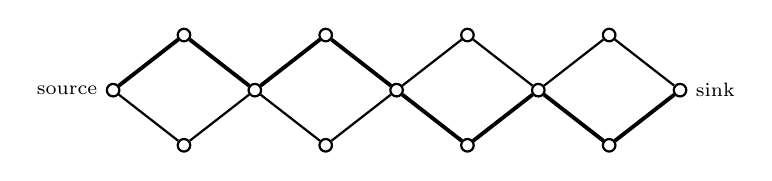
\begin{tikzpicture}[x=0.9cm, y=0.7cm, thick,
    dot/.style={circle, draw, fill=white, inner sep=1.6pt},
    every node/.style={font=\scriptsize}]
  \foreach \x in {0,2,4,6,8} \node[dot] (m\x) at (\x,0) {};
  \foreach \x in {1,3,5,7} {\node[dot] (t\x) at (\x,1) {}; \node[dot] (b\x) at (\x,-1) {};}
  \draw (m0)--(t1)--(m2)--(t3)--(m4)--(t5)--(m6)--(t7)--(m8);
  \draw (m0)--(b1)--(m2)--(b3)--(m4)--(b5)--(m6)--(b7)--(m8);
  \draw[line width=1.4pt] (m0)--(t1)--(m2)--(t3)--(m4)--(b5)--(m6)--(b7)--(m8);
  \node[left=2pt] at (m0) {source};
  \node[right=2pt] at (m8) {sink};
\end{tikzpicture}
\caption{The diamond necklace, with the critical path drawn heavy: up early, down late.  Nodes are lattice points $(x, y)$ with $y \in \{-1,0,1\}$; merges sit on the axis.}
\label{fig:necklace}
\end{figure}

The exhibit is a necklace of diamonds on a coordinate lattice with $y \in \{-1, 0, 1\}$ (Figure~\ref{fig:necklace}).
The edge relation is one analytic rule on the pair of nodes, and because $y$ ranges over $\{-1,0,1\}$ it generates the diamonds on its own:
\begin{equation}
    E\big((x,y),(x',y')\big) \iff x' = x + 1 \;\wedge\; |y' - y| = 1.
\end{equation}
The cost of arriving at $(x', y')$ is $\max\big(y'(K - x'),\, 0\big)$, a non-negative duration (a CPM activity cannot take negative time), so the carrier is \cppinline{unsigned}.
It is $0$ on the axis, so merges are free, positive at the early peaks and late valleys, and clamped to $0$ where $y'(K - x') < 0$; the critical chevron is already non-negative, so the clamp leaves its value unchanged.
Up pays early and down pays late, so the longest path is a chevron, up, up, down, down, of value $3 + 1 + 1 + 3 = 8$.

Listing~\ref{lst:necklace} drives the one closure over three semirings, and Listing~\ref{lst:necklace-ir} is the LLVM IR it emits.

\begin{listing}[htbp]
\caption{One intensional relation, three semirings.  Reachability, the critical-path value, and its edge-cost sensitivity, all from the same \cppinline{semiring_closure} (abridged from the checked-in showcase).}
\label{lst:necklace}
\begin{cpp}
// The analytic rule E((x,y),(x',y')) <=> x'=x+1 & |y'-y|=1, materialised
// (once) as a topological edge sequence -- the extensional form the fold needs.
constexpr auto edges = materialise(nedge);

// Reachability: Boolean semiring, operators defaulted to (OR, AND).
constexpr bool reaches = semiring_closure<bool, Cap>(
    src, sink, edges, [](auto, auto){ return true; });

// Critical path, point-free: collapse the relation to the critical-path
// FUNCTION (a net V -> V), iterate it to the path, fold the path to a scalar.
constexpr FiniteNet<size_t, Cap> pred = annotate<MaxPlus<unsigned long long>, Cap>(src, edges, cost);
constexpr auto path  = critical_path(pred, src, sink);
constexpr long long value = fold(path, 0LL,
    [](long long& acc, Edge e){ acc += cost(e.tail, e.head).val; });
static_assert(value == 8);

// Sensitivity is membership: an edge is critical iff it lies on the path.
static_assert( on_path(path, up_branch(1)));   // up @ x=1: critical
static_assert(!on_path(path, up_branch(7)));   // up @ x=7: floated
\end{cpp}
\end{listing}

\begin{listing}[htbp]
\caption{The emitted IR at \texttt{-O2}: a literal load per witness, no solver and no loop.  These are checked-in fixtures, not a specification.}
\label{lst:necklace-ir}
\begin{cpp}
define i64 @witness_necklace_reachable()            { ret i64 1 }  ; reachable
define i64 @witness_necklace_critical()             { ret i64 8 }  ; critical path
define i64 @witness_necklace_sensitivity_critical() { ret i64 1 }  ; on-path branch
define i64 @witness_necklace_sensitivity_floated()  { ret i64 0 }  ; floated branch
\end{cpp}
\end{listing}

The same closure, driven from the same intensional relation, folds to \texttt{ret i64 1} under the Boolean semiring, to \texttt{ret i64 8} under the tropical semiring, and to \texttt{ret i64 1} and \texttt{ret i64 0} under the tropical dual-number semiring, for an on-path branch and a floated branch respectively.
No solver, no active-set search, and no loop survive in these compile-time witnesses; each is a single literal load.

\paragraph{Compile-time evaluation is optional.}
The closure is an ordinary \cppinline{constexpr} function, so the identical call runs at run time when the endpoints are runtime arguments; the emitted code is then the fold over the edges rather than a constant (the \cppinline{witness_necklace_critical_between} fixture).
The template parameters fix the structure, the semiring and the topology; the value arguments may be static or dynamic.
So the compiler is a partial evaluator~\cite{jones1993partial}: freeze a whole instance and it folds to a constant, freeze only the algebra and a runtime-parametric residual over the data remains.
This is the Juliet Posture's two-way bridge for graphs, and what carries the approach past the fully-static regime.

\paragraph{Sensitivity as the envelope theorem.}
The tropical dual-number instantiation carries $\partial(\mathrm{optimum}) / \partial c_e$ in its tangent.
Because $\max$ selects the winning branch and forwards that branch's derivative, the tangent is $1$ on an edge that lies on the critical path and $0$ on an edge with float, which is exactly the primal flow recovered from the dual by complementary slackness.
This is forward-mode automatic differentiation in Elliott's sense~\cite{elliott2018simple}, the value-and-derivative product $(f, f')$, with the chain rule falling out of the dual-number ring laws, and the \cppinline{Dual<F>} carrier drops into the closure without special-casing.


\section{Compile-Time Cost and Complexity}
\label{sec:evaluation_benchmarks}

The architecture makes a deliberate trade: work is moved out of run time and into the translation-time template engine.
Rather than extrapolate that trade from a single benchmark point, we characterise it in terms of the two parameters that actually govern it, the template instantiation depth and the size of the graph the closure relaxes.

\subsection{Translation-time cost}
\label{sec:translation_overhead_analysis}

The compiler evaluates \cppinline{constexpr} reductions with an abstract-syntax-tree interpreter, so translation-time work is interpretive rather than compiled, and its absolute magnitude is not small.
Its \emph{scaling}, though, is fixed by structure.
The first parameter is the template instantiation depth.
The disciplined fragment of §\ref{sec:jlt_posture} admits no unbounded type-level recursion, so the depth stays bounded and each reduction remains inside a decidable cone rather than diverging; the carrier tower, for instance, is capped at scalar, shape, and quotient axes, a depth of at most three in the current surface.
The second parameter is the size of the graph the closure relaxes.
For the necklace of §\ref{sec:optimization_lp}, each round scans the edge relation once, and an acyclic graph stabilises within a number of rounds bounded by its depth, so the work is polynomial in the edge count $E$.
Composing the two, the translation-time cost is polynomial in the problem size at bounded instantiation depth, precisely because the depth is capped.
An unbounded-depth formulation would forfeit that guarantee; the bounded-depth discipline is what buys both termination and a predictable cost curve, and it is the honest content of the ``severe compilation cost'' the approach is often charged with.

\subsection{Runtime payoff}
\label{sec:runtime_payoff_analysis}

The payoff is structural rather than merely quantitative.
When the graph is declared statically, the reduction resolves the optimum to a typed constant, the critical-path value of §\ref{sec:optimization_lp}, and the backend receives an already constant-folded kernel.
The runtime cost of the resulting binary is therefore $\mathcal{O}(1)$: a literal load, with no solver, no active-set search, and no dynamic indexing left in the emitted code, as the checked-in IR of Listing~\ref{lst:necklace-ir} shows.
The same discipline that folds an empty intersection to \texttt{ret i1 false} (§\ref{sec:ddk_comprehension}) discards the network's redundant constraint paths before code generation, so the emitted pass branches on none of the pruned structure.

This is where the trade pays for itself.
The translation-time cost is $\mathcal{O}(V^{2} + E)$, the $V^{2}$ to materialise the intensional rule over node pairs and the $E$ for the fold, incurred once; the runtime cost of the compiled kernel is $\mathcal{O}(1)$ and is paid on every invocation.
For a workload that runs the same statically-resolved kernel repeatedly, the fixed build-time cost amortises towards zero per invocation, which is the regime the architecture targets: build-time patience exchanged for runtime that is constant by construction, as wanted in real-time embedded control, signal processing, or edge robotics.
The static case is not forced, however: the same kernel accepts a runtime graph as a partially-evaluated residual (Appendix~\ref{app:partial-eval}), so the compile-time versus runtime split is chosen per call site rather than baked into the architecture.

\subsection{The observable is the complexity class}
\label{sec:complexity_class}

Underneath both costs sits a single complexity fact, and it is algebraic rather than empirical.
The necklace has $2^{k}$ distinct source-to-sink paths for its $k$ diamonds, exponential in the graph, yet the closure resolves the critical path in polynomial time and never enumerates a path ($\mathcal{O}(V^{2} + E)$: the $V^{2}$ node-pair materialisation plus the $\mathcal{O}(E)$ fold).
The reason it need not enumerate is the distributivity of the semiring, $a \otimes (b \oplus c) = (a \otimes b) \oplus (a \otimes c)$: distributivity is exactly what lets the sum over all paths be computed as a fold over the $V$ nodes, which is dynamic programming stated as an axiom.
So the \cppinline{IsSemiring} gate of §\ref{sec:optimization_lp} is not only the correctness condition; its distributive law is the \emph{complexity guarantee}, and the polynomial residual the compiler ships is a theorem about the algebra rather than a measured quantity.

This is why the paper reports no benchmark.
A single measured cost curve fixes one machine, one toolchain, and one problem size, none of which the structural claim depends on.
That claim, that the exponential path space collapses to a polynomial fold and that a statically-declared instance collapses further to $\mathcal{O}(1)$, is portable across any conforming C++23 optimiser that constant-folds \cppinline{constexpr}, and it would only be obscured by pinning it to one observation.
The observable is the move to a sensible complexity class, and that is the whole of the empirical claim.

% ============================================================
\section{Discussion and Future Work}
\label{sec:discussion}
% ============================================================

Two limitations of the present artefact point in the same direction.
First, the real numbers are handled only rudimentarily.
\texttt{dedekind}'s $\mathbb{R}$ is a Dedekind-cut carrier whose comparison is only semi-decidable, and most numeric work still bottoms out in IEEE \cppinline{double}, which is not cleanly algebraic: rounding defeats associativity and \texttt{NaN} punctures the order.
Second, the optimisation and differentiation exhibits fold at compile time only over exact carriers such as $\mathbb{Q}$ and $\mathbb{Q}[\varepsilon]/(\varepsilon^2)$, not over the floating-point types production code runs on.

A natural way to reconcile the two is a \emph{controlled boundary}, in the sense of staged, multi-stage programming~\cite{taha2000metaml}.
Write the computation as a symbolic algebraic expression over an exact ring where the laws genuinely hold, let $\mathbf{Jlt}$ simplify and prune it at translation time, and only then lower the residual to IEEE floating-point for execution.
The rewrites are sound because they happen on the exact ring.
The lossy step is a single explicit evaluation map at the boundary, not a silent assumption threaded through every operation.
This is the ring-swap machinery the \cppinline{Dual<F>} sensitivity exhibit (§\ref{sec:optimization_lp}) already uses in miniature, generalised from computing a derivative exactly to computing the whole expression exactly and rounding once.
Whether the type system can carry that boundary crossing as a first-class, mechanically-checked seam rather than a convention is the question we would pursue next.

A complementary direction widens the family of structural specialisations the compiler recognises (§\ref{sec:ddk_comprehension}) toward a law-indexed reduction surface: gating the collapse rules on algebraic-law concepts such as \cppinline{IsMonoid} and \cppinline{IsSemilattice} rather than on named carriers.
Rice's theorem forecloses a fully general reducer.
The family of law-carrying specialisations, however, has no obvious ceiling short of it.

% ============================================================
% ============================================================
\printbibliography

\appendix


%%%
\section{Partial Evaluation on the Analytic Necklace}
\label{app:partial-eval}

The diamond necklace of §\ref{sec:optimization_lp} is an \emph{analytic} graph: its edges are a rule on a pair of nodes, $E((x,y),(x',y')) \iff x' = x+1 \wedge |y'-y| = 1$, with no intrinsic size.
The closure materialises a finite window of it as a budget, and where its endpoints are fixed decides how much of the computation the compiler performs.

\paragraph{Endpoints at compile time: full collapse.}
When source and sink are compile-time constants, the whole reduction is a constant expression and folds to a literal, the \texttt{ret i64 8} of Listing~\ref{lst:necklace-ir}.
Nothing of the graph, the semiring, or the traversal survives into the binary.

\paragraph{Endpoints at run time: a specialised residual.}
When source and sink instead arrive as runtime arguments, the identical \cppinline{semiring_closure} cannot fold, and the emitted code is its \emph{residual}.
That residual is not a generic solver: the semiring is specialised in ($\oplus = \max$ is a \cppinline{select}, $\otimes = {+}$ is an \cppinline{add}), the topology rule is the inlined coordinate decode, and the cost formula $y'(K-x')$ is inlined arithmetic; what remains parametric is only the pair of runtime endpoints.
This is partial evaluation~\cite{jones1993partial} in the precise sense: freezing the structure and leaving the data specialises one expression into a family of optimised kernels, one per graph query, with the query itself as the runtime-parametric continuation.

\begin{listing}[htbp]
\caption{The same necklace closure, two call sites (checked-in witnesses).  Static endpoints fold to a constant; runtime endpoints leave a specialised residual.}
\label{lst:partial-eval}
\begin{cpp}
// Endpoints static  -> constant expression -> ret i64 8 (full collapse).
constexpr auto opt = semiring_closure<MaxPlus<unsigned long long>, Cap>(
    SRC, SINK, edges, cpm_cost);            // SRC, SINK literals

// Endpoints runtime -> residual: the fold over the edges, max/add inlined,
// indexed by (source, sink); no generic solver, no dispatch.
int64_t critical_between(std::size_t source, std::size_t sink) {
  if (source >= Cap || sink >= Cap) return -1;   // out-of-range query
  const auto d = semiring_closure<MaxPlus<unsigned long long>, Cap>(
      source, sink, edges, cpm_cost);            // source, sink runtime
  return d.finite ? d.val : -1;                  // unreachable -> -1, not 0
}
\end{cpp}
\end{listing}

The residual is the fold over the edge sequence rather than a straight-line kernel: the optimiser keeps the loop that threads the potential, specialised but not flattened.
The point the two call sites make is that the collapse is optional and the boundary is the programmer's to place.

%%%
\section{An Elementary Theory of the Category of Sets}
\label{sec:etcs}

With a deterministic, structurally-typed substrate established in Section~\ref{sec:jlt_posture}, mathematical sets can be bootstrapped inside the type system. Here, we aim to model both the syntax and the semantics of mathematical set-builder notation in executable \textbf{Jlt}, hoping to achieve a system that lends itself to the expression and subsequent evaluation of precisely those kinds of problems that one might also encounter in a pure math blackboard setting.

A common implementation approach follows material Zermelo-Fraenkel (ZF) set theory, where the discussion starts from an element membership relation $\in$ acting on a cumulative universe of sets. Implementations such as \texttt{std::set} use this as a starting point and model sets as \textit{extensional memory containers}. The identity of a set is determined by explicitly enumerating its members in physical allocations, and membership is evaluated by traversing a data structure (e.g., a balanced binary search tree). This approach exhibits prohibitive shortcomings when applied to algebraic and engineering problems: for example, it cannot natively model infinite sets like the natural numbers $\mathbb{N}$, or non-enumerable continuous intervals over the real numbers $\mathbb{R}$. As a result, both the structural guarantees a compiler can infer and the optimizations it can perform on such problems are severely restricted.

By contrast, the \textit{structural categorical comprehension} view pioneered by William Lawvere~\cite{lawvere1964etcs} abandons element-centric containment. Instead, it defines a set entirely through its relational behavior using objects and functions (\textit{morphisms}). In this framework, we do not ask what an element \textit{is} internally; we ask how it behaves under functional composition. Lawvere’s Elementary Theory of the Category of Sets (\textbf{ETCS}) posits that the category of sets (\textbf{Set}) is a well-pointed, Cartesian Closed Category with a subobject classifier, a natural numbers object, and the axiom of choice.

To bridge this abstract mathematical formalism with systems-programming primitives, we translate the foundational axioms of ETCS into explicit C++23 type-predicates (\texttt{concept IsSet}) distributed across six localized compile-time partitions:

\subsection{Small Categories (\texttt{:small} partition)}
\begin{itemize}
    \item \textbf{Axioms of Categories \& Smallness:}
    \begin{enumerate}
        \item \textit{Category:} a collection of objects and arrows (morphisms) closed under an associative composition with identities.
        \item \textit{Smallness:} both collections are \emph{sets}, not proper classes. This holds \emph{by construction}, since the objects and arrows are the value-sets of single C++ types (\cppinline{Cat::Species} and \cppinline{Cat::Arrow}), and a type's value-set is a set in the metatheory. (Requiring only the hom-collection to be a set gives the weaker notion of a \emph{locally small} category.)
    \end{enumerate}
    \item \textbf{C++ Reification:} The \cppinline{concept IsSmallCategory} gates the structure. Per $\mathbf{Jlt}$~\ref{sec:jlt_posture}, objects are \cppinline{std::regular} carriers. Morphisms are values of a single arrow type satisfying \cppinline{concept IsArrow}, with \texttt{::Domain} and \texttt{::Codomain} typedefs and a callable \cppinline{f(x)} from the domain into the codomain. Composition is the overloaded \cppinline{operator>>}, with the identity laws \cppinline{id >> g == g} and \cppinline{f >> id == f} discharged as overloads; identity arrows come from an \cppinline{id_c(x)} factory.
    \item \textbf{Explanatory Note:} Instead of data-hiding containers, a ``set'' at this entry rung is simply a well-behaved C++ type acting as a domain, and a ``function'' is a side-effect-free arrow mapping inputs to outputs. In its single-object mode, with the carrier type as the sole object and its arrows as endomorphisms, composition makes the category a \textbf{monoid} (a one-object category). These are exactly the endomorphism loops drawn on each carrier hub of Figure~\ref{fig:hub-spoke-bnz}.
\end{itemize}

\subsection{Cartesian Categories (\texttt{:limit} partition)}
\begin{itemize}
    \item \textbf{Axioms of Terminal Object \& Finite Products:}
    \begin{enumerate}
        \item \textit{Terminal Object:} There is a terminal object $1$, characterised purely by its universal property: every set $A$ has exactly one arrow $A \to 1$.
        \item \textit{Binary Products:} For any sets $A$ and $B$ there is a product $A \times B$ with projections $\pi_1: A \times B \to A$ and $\pi_2: A \times B \to B$, universal in that every pair $f: X \to A$, $g: X \to B$ factors through a unique $\langle f, g\rangle: X \to A \times B$.
    \end{enumerate}
    \item \textbf{C++ Reification:} \cppinline{concept IsTerminalObject} and \cppinline{concept IsProduct} gate the structure, and the standard library satisfies them out of the box: \cppinline{std::monostate} \emph{is} the terminal object (exported as \texttt{One}), and \cppinline{std::pair} \emph{is} the binary product, with projections $\pi_1 / \pi_2$ reading \cppinline{.first} / \cppinline{.second}. The universal factorisation $\langle f, g\rangle$ is the one piece \cppinline{std} does not provide; the library supplies it as the default \cppinline{mediate_product} arrow.
    \item \textbf{Explanatory Note:} This layer turns relational coordinate tables into type-safe tuples. The terminal object lets us define ``elements'' of a set $A$ structurally, as arrows \texttt{One} $\to A$.
\end{itemize}

\subsection{Cartesian Closed Categories (\texttt{:cartesian} partition)}
\begin{itemize}
    \item \textbf{Axiom of Exponentials:} For any sets $A$ and $B$ there is an exponential $B^A$: the set of functions $A \to B$ with an evaluation map $\mathrm{eval}: B^A \times A \to B$, universal in that every $f: X \times A \to B$ factors through a unique $\mathrm{curry}(f): X \to B^A$ (the adjunction $(-\times A) \dashv (-)^A$).
    \item \textbf{C++ Reification:} The exponential $B^A$ is the internal hom, whose inhabitants are the functions $A \to B$. It is required by \cppinline{concept IsCartesianClosed} via \cppinline{concept IsExponential}. The adjunction arrows \cppinline{curry} / \cppinline{uncurry} / \cppinline{eval} are library-provided.
    \item \textbf{Explanatory Note:} This licenses function \textit{Currying} at compile time via the \cppinline{constexpr} lambdas. It guarantees that functions are first-class citizens that can be passed, stored, and transformed by other functions without dropping out of the type-checking engine.
\end{itemize}

\subsection{Elementary Topoi (\texttt{:topoi} partition)}
\begin{itemize}
    \item \textbf{Axioms of Subobject Classifier \& Equalizers:}
    \begin{enumerate}
        \item \textit{Subobject Classifier:} a truth-value object $\Omega$ with an element $\mathrm{true}: 1 \to \Omega$ such that every mono $S \hookrightarrow A$ arises as the pullback of $\mathrm{true}$ along a \emph{unique} characteristic map $\chi: A \to \Omega$.
        \item \textit{Equalizers:} for parallel arrows $f, g: A \to B$, the subobject $\{x \in A \mid f(x) = g(x)\}$.
    \end{enumerate}
    \item \textbf{C++ Reification:} The classifier $\Omega$ is Boolean. What a carrier plugs in is the codomain of its (possibly partial) characteristic map, fixed by a \emph{logic species} \cppinline{L} (the code names this codomain \cppinline{L::Omega}). \cppinline{ClassicalLogic} gives $\mathbb{B}$ (\cppinline{bool}), a total map; \cppinline{TernaryLogic} gives the lifted Boolean (\cppinline{Ternary}, $\mathbb{B}+\text{U}$, under strong-Kleene connectives), the codomain of a partial $\chi$. \cppinline{concept IsLogicalSpecies} gates such a species; the predicate of a \cppinline{Set<T, L, P>} is $\chi$, and \cppinline{concept IsSubobject} recognises it. Which codomain a carrier receives is the decidability split of Section~\ref{sec:ddk_etcs}: $\mathbb{B}$ where membership is decidable, the lifted Boolean where it is not. Equalizers are named by \cppinline{concept IsEqualizer}, the subobject solving $f = g$.
    \item \textbf{Explanatory Note:} An \textit{intensional} set is a rule, not an array. Testing $x \in S$ evaluates $\chi(x)$ instead of searching memory.
\end{itemize}

\subsection{Concrete Topoi (\texttt{:concrete} partition)}
\begin{itemize}
    \item \textbf{Axioms of the Powerset Monad \& Elementality:} Every set $A$ maps functorially to its powerset $\mathcal{P}(A)$ via a unit morphism $\eta_A: A \to \mathcal{P}(A)$.
    \item \textbf{C++ Reification:} Expressed via the \texttt{SetAsProduct} layout template, which combines a raw underlying C++ data type primitive with its corresponding logical evaluator lambda.
    \item \textbf{Explanatory Note:} This layer implements a faithful \textit{forgetful functor} $U$, which strips away structural categorical formatting to expose underlying raw C++ hardware types when evaluation is explicitly required. Constructing lazy evaluation pipelines (e.g., using \texttt{std::views::transform}) functions as monadic composition, chaining transformations without intermediate memory allocations.
\end{itemize}
Axiom 9: Power Set / Exponential Restriction (\(\beth _{1}\)). For any set X, there exists an object \(\mathcal{P}(X)\) classifying its subobjects. By Cantor’s theorem (Lawvere’s Fixed-Point Theorem), this explicitly bounds the cardinality of classical constructible sets in the base theory below the second transfinite cardinal. Russell's paradox is ruled out by construction. Library Reification: Restricts carrier predicates from modeling uncountably infinite domains beyond the continuum \(\beth _{1}\), avoiding type-system divergence and ensuring all logical intersections resolve during template translation.

\subsection{Set-Modeling Topoi (\texttt{:etcs} partition)}
\begin{itemize}
    \item \textbf{Axioms of Well-Pointedness, Infinity, and Choice:}
    \begin{enumerate}
        \item \textit{Well-Pointedness:} If two functions $f, g: A \to B$ are distinct, there must exist a single element $x: 1 \to A$ such that $f(x) \neq g(x)$.
        \item \textit{Infinity:} There exists a Natural Numbers Object (NNO) $\mathbb{N}$ that enables primitive recursion without structural loops.
        \item \textit{Choice:} Every surjective function has a right inverse section.
    \end{enumerate}
    \item \textbf{C++ Reification:} Enforced via the \texttt{IsSet} concept constraint. Well-pointedness enforces referential transparency and forbids hidden mutable states. Infinity is preserved by generating strict element-level partial orderings via \texttt{std::three\_way\_comparable} rather than managing physical loop limits.
    \item \textbf{Explanatory Note:} The NNO lets the library model \textit{transfinite spaces} (e.g., continuous mathematical boundaries or infinite sequence generators) lazily. The Axiom of Choice ensures that the template engine can constructively find or instantiate witness values for non-empty subset selections during compile-time verification passes.
\end{itemize}

%%% 
\section{From Cardinality Pruning to Type-Directed Collapse}
\label{sec:gap}
%%% 

Step back from the showcases for a moment. What is the pattern? In every
one of them we started with an intensional set---a predicate---and we
ended with a named extensional object whose \emph{type} carries the
answer: $\varnothing$, a singleton, an order interval of known
cardinality, an LP vertex. The collapse is not incidental; it is a
rewrite rule, running inside the type system, at translation time. To
make the claim precise, we first formalise ``how much the compiler
knows about a set'' as a lattice, then state the theorem as monotone
motion up that lattice.

\begin{definition}[Computability tier]
\label{def:computability-tier}
For a compile-time set $S$ over an ambient carrier $T$, the
\emph{computability tier} is the triple
\[
  \mathcal{T}(S) \;=\; \bigl(\,\mathsf{R}(S),\; \mathsf{L}(S),\; \mathsf{K}(S)\,\bigr)
  \;\in\; \{\mathrm{Int},\mathrm{Ext}\} \times \{\mathrm{K3},\mathrm{Cl}\} \times \{\mathrm{Opq},\mathrm{Elt}\}
\]
whose components are the \emph{representation} tier ($\mathsf{R}$:
intensional vs.\ extensional, i.e.\ predicate vs.\ elements-in-type),
the \emph{logic} tier ($\mathsf{L}$: Kleene three-valued vs.\
classical two-valued membership), and the \emph{knowledge} tier
($\mathsf{K}$: elements opaque vs.\ carried in the type). Each axis
carries the order $\mathrm{Int} \preceq \mathrm{Ext}$,
$\mathrm{K3} \preceq \mathrm{Cl}$,
$\mathrm{Opq} \preceq \mathrm{Elt}$; the product order is
componentwise. The resulting Boolean lattice $(\mathcal{T}, \preceq)$
has bottom $\bot = (\mathrm{Int},\mathrm{K3},\mathrm{Opq})$ (``a raw
predicate over a floating-point carrier with no inhabitants known'')
and top $\top = (\mathrm{Ext},\mathrm{Cl},\mathrm{Elt})$ (``a named
finite set whose members are template parameters and whose membership
is decidable'').
\end{definition}

Every showcase of Section~\ref{sec:ddk_comprehension} is a motion inside this
lattice. The empty-halfspace reductions of Showcase~3 go $(\mathrm{Int},\mathrm{K3},\mathrm{Opq}) \mapsto \top$
in one step (the result is $\varnothing$); the cardinality-1 reduction
of Showcase~4 does the same. The
reductions never slide downward. With that in hand:

\begin{theorem}[Type-Directed Collapse, totally-ordered 1D case]
\label{thm:type-directed-collapse-1d}
Let $T$ be a totally ordered carrier, and let
\[
  P_i(x) \;=\; (x \ge a_i), \quad i = 1, \dots, m,
  \qquad
  Q_j(x) \;=\; (x \le b_j), \quad j = 1, \dots, n,
\]
be lower-bound and upper-bound halfspace predicates over $T$ whose
pivots $a_i, b_j \in T$ are carried at the type level as non-type
template parameters. Define the effective bounds
$a^\star \coloneqq \max_i a_i$ if $m \ge 1$ and $a^\star \coloneqq
\bot$ if $m = 0$, and $b^\star \coloneqq \min_j b_j$ if $n \ge 1$
and $b^\star \coloneqq \top$ if $n = 0$ (where $\bot, \top$ denote
the carrier's bottom and top elements, taken as
$\pm\infty$-style sentinels when $T$ is unbounded). Then the meet
\[
  S \;=\; \bigcap_{i=1}^{m} \{x \in T \mid P_i(x)\}
        \;\cap\;
        \bigcap_{j=1}^{n} \{x \in T \mid Q_j(x)\}
\]
is resolved at compile time to exactly one of:
\begin{enumerate}
  \item $\varnothing$, when $a^\star > b^\star$;
  \item a \cppinline{Singleton<v>}, when $T$ is integral and
        $a^\star = b^\star = v$;
  \item an \cppinline{OrderInterval}~$[a^\star, b^\star]$
        otherwise.
\end{enumerate}
\end{theorem}

\begin{figure}[htbp]
\centering
\begin{tikzcd}[column sep=3em, row sep=4em, ampersand replacement=\&]
\& \mathrm{Halfspace}\langle x \geq a^\star\rangle \,\cap\, \mathrm{Halfspace}\langle x \leq b^\star\rangle
  \arrow[dl, "{[a^\star < b^\star]}"']
  \arrow[d, "{[a^\star = b^\star,\, T \text{ integral}]}"']
  \arrow[dr, "{[a^\star > b^\star]}"] \& \\
\mathrm{OrderInterval}\langle a^\star, b^\star\rangle \& \mathrm{Singleton}\langle v\rangle \& \mathrm{EmptyPredicate}\langle T\rangle
\end{tikzcd}
\caption{The 1D type-directed collapse as a diagram chase (Theorem~\ref{thm:type-directed-collapse-1d}).
The meet of the effective lower- and upper-bound halfspaces resolves at compile time into exactly one of three typed constants, selected by the side condition on the pivots: an \cppinline{OrderInterval<a*, b*>} for the generic bounded case ($a^\star < b^\star$); a \cppinline{Singleton<v>} for the degenerate equality case ($a^\star = b^\star = v$) \emph{when $T$ is integral} (the integrality guard from Theorem~\ref{thm:type-directed-collapse-1d} case 2; on a non-integral $T$ the equality case stays in the (degenerate) \cppinline{OrderInterval<a*, a*>} branch instead); and \cppinline{EmptyPredicate<T>} (lifted to $\varnothing$ at the topos level) for the contradiction case ($a^\star > b^\star$).
The diagram commutes on elements: $x$ inhabits the source meet iff $x$ inhabits the target type the side-condition selects.
Implementation hook: the meet is realised by \cppinline{structured_and(Halfspace<...,Upward,...>, Halfspace<...,Downward,...>)} in \texttt{dedekind.order:halfspace}, which case-splits the pivot comparison at compile time and returns the corresponding typed constant directly; the empty-result type \cppinline{EmptyPredicate<T>} lives in \texttt{dedekind.order} and lifts to \cppinline{Ø<T,L>} in \texttt{dedekind.sets:boundaries}.
Mechanically witnessed by Showcase~3 (\cppinline{EmptyPredicate<T>} branch, \texttt{showcase\_03\_halfspace\_contradiction.cpp}) and Showcase~4 (\cppinline{Singleton<6>} branch, the cardinality-1 reduction in Listing~\ref{lst:pruning}); both fold to constant IR returns under \texttt{-O2}, as Listing~\ref{lst:pruning_ir} demonstrates for the empty-meet branch.}
\label{fig:type-directed-collapse-1d}
\end{figure}

\begin{proof}
By induction on $m + n$.

\smallskip
\noindent\emph{Base case} ($m + n = 0$): no constraints; $S = T$,
which is the order interval $[\bot, \top]$ (case 3) by the boundary
convention.

\smallskip
\noindent\emph{Inductive step.} Assume the claim holds for $k$ total
constraints. Add one more; without loss of generality (by the
symmetry between lower and upper bounds) take it to be a fresh
lower-bound predicate $P_*(x) = (x \ge a_*)$. The inductive
hypothesis gives a reduced form $S_k$ of one of the three shapes.
Form $S = S_k \cap \{x \mid x \ge a_*\}$. Two compile-time
comparisons of $a_*$ against the bounds of $S_k$ (where present)
suffice:

\begin{itemize}
  \item \textbf{Redundant.} If $S_k$ has lower bound $a$ and
        $a_* \le a$, then $\{x \mid x \ge a_*\} \supseteq S_k$ and
        $S = S_k$; the form is preserved.
  \item \textbf{Tightening.} If $S_k$ is the interval $[a, b]$ (or
        unbounded above) and $a < a_* \le b$ (or no upper bound),
        then $S = [a_*, b]$ in case 3; if $T$ is integral and
        $a_* = b$, then $S = \{a_*\}$ (case 2).
  \item \textbf{Contradicting.} If $S_k$ has upper bound $b$ and
        $a_* > b$, or if $S_k$ is already $\varnothing$, then
        $S = \varnothing$ (case 1).
\end{itemize}

\noindent
The same case-split, with rôles of $a_i$ and $b_j$ exchanged,
discharges the symmetric upper-bound addition. Each case lands in
one of the three forms, completing the induction.
\end{proof}

\paragraph{Theorems for free.}
The structural shape of Theorem~\ref{thm:type-directed-collapse-1d}
is Wadler's \emph{Theorems for Free!}~\cite{wadler1989theorems}
move at the algebraic register. Wadler showed that polymorphic
types in the typed lambda calculus discharge a class of theorems by
parametricity alone, with no further proof obligation on the
caller. Here, the analogous discharge runs from \emph{carrier-axiom
declaration} (\cppinline{HasTotalOrderOperators<T>} +
\cppinline{IsTotallyOrdered<T>}, plus the integral-carrier
witness when case 2 is to fire) to a carrier-level reduction of any
finite intersection of half-line constraints. The engineer's
honesty obligation is the axiom set; the collapse is
type-level free. The proof above is one demonstration that the
discharge is mechanical---the inductive argument does not depend on
which carrier or which pivot type, only on the axiom slots being
filled.

\paragraph{Existential anchor.}
The theorem is realised in the library by witnesses that
materialise at the static-assertion layer; the canonical exhibit on
$\mathbb{N}$ is the typed-constant collapse
\[
  \{x \in \mathbb{N} \mid x \ge 2\} \,\cap\, \{x \in \mathbb{N} \mid x \le 5\}
  \;\longrightarrow\;
  \texttt{OrderInterval}\langle 2, 5\rangle,
\]
checked at compile time. Section~\ref{sec:ddk_comprehension} catalogues these
witnesses; the LLVM~IR fixtures pin the resulting machine-code
collapse downstream of the type-level reduction.

\begin{conjecture}[Type-Directed Collapse, n-dimensional generalisation]
\label{conj:type-directed-collapse-nd}
Let $T_1, \dots, T_d$ be totally ordered carriers and let
$\{P_k\}_{k=1}^{N}$ be halfspace predicates over the product
$T_1 \times \dots \times T_d$ whose pivots are carried at the type
level. The meet
\[
  S \;=\; \bigcap_{k=1}^{N} \{(x_1, \dots, x_d) \mid P_k(x_1, \dots, x_d)\}
\]
admits a compile-time reduction to a typed normal form
generalising the three cases of
Theorem~\ref{thm:type-directed-collapse-1d} (empty, vertex-singleton,
or a polytope record carrying its active constraint set), under a
suitable axiom set on the product carrier (total order per axis,
closure of the meet under the product, and a vertex-enumeration
discipline for the polytope case). Writing $S_k$ for the
single-constraint set, the reduction is monotone up the
computability-tier lattice:
\[
  \mathcal{T}(S) \;\succeq\; \bigvee_{k} \mathcal{T}(S_k),
\]
and strictly so on at least one axis in every case the library
exhibits.

\smallskip
\noindent\emph{Status of claim.} This conjecture is \emph{not}
proved in the paper. It is supported by the same exhibition pattern
as the 1D theorem: each case is checked into the library as a
\cppinline{static_assert}/\cppinline{STATIC_CHECK} witness and,
where relevant, as an LLVM~IR fixture that fails CI on optimiser
drift (see Section~\ref{sec:ddk_comprehension}). A general inductive proof over
dimensions $d$ is left open.
\end{conjecture}

\begin{corollary}[Iterated collapse]
\label{cor:iterated-collapse}
Any finite composition of type-directed-collapse reductions is itself
monotone up $\mathcal{T}$. In particular, no sequence of library
operations can ever return a set that is \emph{less} decidable than
its inputs.
\end{corollary}

So: not ``a faster way to do set algebra'', but a rewrite rule that
happens to live in the C++ type system, and whose action is
monotone-ascending in a lattice of decidability. The halfspace case is
the smallest non-trivial instance we know how to prove mechanically.
Four further axes appear to obey the same pattern; the project tracker
carries one existential proof per axis---one worked instance, one IR
fixture, one compile-time witness---rather than a general framework.
We would rather ship one reduction that fully collapses than four
sketches that do not.

% Tracker cross-reference for maintainers (invisible in PDF):
%   Carrier tightening      -> issue #362
%   Smooth optimization     -> issue #363
%   Linear programming      -> issue #364  (demonstrated here)
%   Lattice-law rewriting   -> issue #365
\begin{itemize}
  \item \textbf{Carrier tightening.} Intersecting a subset of
    $\mathbb{N}$ with a subset of $\mathbb{R}$ should land in $\mathbb{N}$:
    the carrier lattice contributes its own structural reduction via the
    existing canonical embeddings (\cppinline{embed_uint_sint_},
    \cppinline{embed_ℚ_ℝ}, \ldots).
  \item \textbf{Smooth optimization.} The stationary set
    $\{x \mid \nabla f(x) = 0\}$ for a quadratic $f$ collapses to a
    \cppinline{Singleton<x*>} with the minimizer in the template parameter.
    Same reduction pattern, applied at the extremum operator.
    \emph{Scope note:} the polytope / linear-programming domain is not
    incidental.  Active-set enumeration over halfspaces is
    constructively bounded at compile time precisely because halfspaces
    have finite combinatorial structure; non-polyhedral domains
    (KKT-stationary-point search over arbitrary smooth $f$) require
    symbolic root-finding which does not terminate at template-
    instantiation time.  Quadratic $f$ is the worked-instance
    boundary; non-linear extensions are post-paper work tracked
    under \#363.
  \item \textbf{Network critical path, a linear-programming dual}
    (demonstrated in Section~\ref{sec:optimization_lp}).
    The critical path of a directed acyclic network reduces, at
    compile time, to a typed constant; the same closure over a
    dual-number carrier yields edge-cost sensitivity with no extra code
    path: the solver is the compiler.
  \item \textbf{Lattice-law rewriting.} Distributivity and
    absorption applied at the type level rewrite
    $(A \cup B) \cap \lnot A$ to $B \cap \lnot A$ \emph{before} local
    reduction rules fire, exposing collapses that a purely local analysis
    would miss.
\end{itemize}

Each axis sits on the foundation shared with Section~\ref{sec:ddk_comprehension}: NTTP
predicates, structured \cppinline{operator&} dispatch, and the computability
tiers visible in the showcases. Taken together they sketch a program of
which the present halfspace reductions are one installment.

The polynomial-calculus exhibit (companion-repository
\texttt{:polynomial} / \texttt{:ftc} partitions) belongs to the same
family but at the \emph{function} layer: a polynomial reduced under
\cppinline{derive} (a ring homomorphism) or a numerical integrator
yields another intensional object whose identity with a target is
discharged by the compiler.

\paragraph{Scaling beyond atomic carriers via structure-preserving combinators.}
The same partition---atoms below, runtime above---governs the
linear-algebra surface the paper exhibits at the $2 \times 2$ scale.
The library ships \texttt{Invertible2x2}, \texttt{Matrix2x2V},
\texttt{Vec2V} as statically-validated atoms; larger systems are
\emph{not} reached by inflating the atom (we do not aim for
$n \times n$ inversion in templates), but by composing atoms through
\emph{structure-preserving combinators} that propagate the
invariants up.  \texttt{DirectSum<A, B>} carries invertibility from
its factors to the block-diagonal whole and is shipped today;
$4 \times 4$ invertibility is therefore already a one-combinator
step from the $2 \times 2$ atom, with $(A \oplus B)^{-1} =
A^{-1} \oplus B^{-1}$ exact over $\mathbb{Q}$ and verifiable by
\texttt{static\_assert}:

% Source:
% src/test/cpp/modules/dedekind/linear_algebra/matrix_test.cpp
\begin{cpp}
TEST_CASE("linear_algebra:matrix --- Tier 1: "
          "DirectSum preserves invertibility") {
  constexpr Invertible2x2<Rat, Rat{1L}, Rat{2L},
                          Rat{3L}, Rat{4L}> block_M{};
  // 90° rotation over ℚ.
  constexpr Invertible2x2<Rat, Rat{0L}, Rat{-1L},
                          Rat{1L}, Rat{0L}> block_rot{};
  constexpr DirectSum<decltype(block_M),
                      decltype(block_rot)> ds{};
  constexpr auto ds_inv = ds.inverse();

  using IdentityDirectSum =
      DirectSum<Identity2x2<Rat>, Identity2x2<Rat>>;
  STATIC_CHECK(ds * ds_inv == IdentityDirectSum{});
  STATIC_CHECK(ds_inv * ds == IdentityDirectSum{});
}
\end{cpp}

\noindent \texttt{BlockUpperTriangular<A, B, D>} extends the same
propagation to triangular blocks under a degenerate-Schur condition
(also shipped, also testable as a single \texttt{static\_assert}); a
future Kronecker combinator preserves orthogonality and lattice
structure compositionally.  Each combinator is itself a small
structurally-checked unit; their composition gives $2^k \times 2^k$
matrices whose invariants follow by induction without exponential
blowup in the templates.  The remaining roadmap items
% Backlog: issues #366 (block-Schur invertibility recursion, full
% non-degenerate case), #368 (catalog of well-behaved matrix
% carriers --- orthogonal, rotation, diagonal), #369 (structure-
% preserving combinators including Kronecker).
fall out of the same Axiomatic-Systems-Programming discipline rather
than requiring a different paradigm, and are tracked in the project
backlog rather than discharged here.  The $2 \times 2 \to 4 \times 4$
step is a witness, not a promise; everything beyond is the natural
recursion of the same combinator pattern.

\paragraph{Carrier choices, error messages, ergonomics.}
The carrier-vs-overflow trade-offs are catalogued in
Section~\ref{sec:carrier-rosetta}'s Rosetta tables: showcases default
to \cppinline{Rational<SignedExtensionalCardinal<>>} (exact, no
silent overflow); programmers who trade exactness for native
performance pick a primitive row and accept the named failure mode
(signed-overflow UB on \cppinline{int}; non-associative rounding on
\cppinline{float}/\cppinline{double}).  The combinators of
Section~\ref{sec:ddk_comprehension} bind to \cppinline{HasRingOperators}
rather than any particular carrier, so the swap is a one-line change
at the \cppinline{using} declaration.  Error messages, by contrast,
are a more universal C++ pain: a failed \texttt{static\_assert} in a
deep reduction can produce a multi-page expansion trail that no
library can fully repair.  The realistic ambition is to \emph{fail
fast at the named axiom} --- the first message the reader sees should
be the predicate that genuinely broke, not the cascade of downstream
failures it triggered.  The library structures concept ladders so
that each rung adds a single named requirement, and uses targeted
\cppinline{static_assert} messages inside internal reductions, so a
violation surfaces at the smallest witness rather than deep inside
overload resolution.\footnote{Worked diagnostic: a rank-deficient
\cppinline{Invertible2x2<Rat, 1, 2, 2, 4>} input produces a single
named message (\texttt{Invertible2x2 requires full rank: a*d - b*c
!= 0}) at the \texttt{static\_assert} site with one \texttt{note}
pointing at the instantiation, no substitution-failure cascade.  The
predicate sits inside the class body as a literal
\texttt{static\_assert} rather than as a \cppinline{requires}-clause
to be probed, so the diagnostic fires at the named axiom directly.}

In short: the compiler wall has a predictable shape---depth, steps,
combinatorics, numeric range, diagnostics---and each is either
pushable by a flag, avoidable by staying within the instance regime
for which this technique is intended, or a known limitation we do not
claim to have solved. The paper's contribution lies entirely to the
left of that wall.

\paragraph{Frictions: where C++23 and IEEE numerics break the chain.}
The axioms cannot always be discharged. The friction points encountered while
building the library are observational, not advocacy, and each is
pinned at a concrete file in source (with the relevant lines flagged
in the corresponding partition's witness blocks) so a reader can
verify the mechanism rather than take the claim on faith.
\emph{Integer-promotion shape mismatch}: \cppinline{bool + bool} and
\cppinline{bool * bool} return \cppinline{int} rather than
\cppinline{bool}; \cppinline{unsigned short + unsigned short} /
\cppinline{unsigned short * unsigned short} and
\cppinline{unsigned char + unsigned char} /
\cppinline{unsigned char * unsigned char} likewise promote to
\cppinline{int}. The functor surface
(\cppinline{std::plus<bool>}, \cppinline{std::multiplies<unsigned short>})
returns the carrier by signature, but the literal \cppinline{+} /
\cppinline{*} operator surface does not (witnessed at
\texttt{algebra/ring.cppm}, \texttt{algebra/field.cppm},
\texttt{morphologies/uint.cppm}, \texttt{order/lattice.cppm}).
\emph{Signed-overflow UB defeats $\mathbb{Z}$}: \cppinline{int} /
\cppinline{long} / \cppinline{long long} carry the literal ring
operator surface
(\cppinline{HasRingOperators<int>} fires) but \emph{not} the
axiomatic ring witness, because closure-under-arithmetic fails as a
stable axiom under signed-overflow UB; the negative pins
\cppinline{!IsArithmeticAdditiveGroup<int>} and
\cppinline{!category::IsRing<int, std::plus, std::multiplies>} at
\texttt{morphologies/sint.cppm} make the rejection mechanical.
\emph{IEEE 754 breaks reflexivity}: \cppinline{NaN <= NaN}
evaluates to \cppinline{false}, so
\cppinline{is_reflexive_v<double, std::less_equal<>>} is deliberately
not registered, and \cppinline{!IsTotallyOrdered<double>},
\cppinline{!IsTotallyOrdered<long double>}, and
\cppinline{!category::IsRing<double, std::plus, std::multiplies>}
all hold (\texttt{morphologies/floating\_point.cppm} +
\texttt{order/total.cppm}); the operational ordered-field reading
survives via \cppinline{IsOrderedField<double>} in
\texttt{morphologies/archimedean.cppm}.
\emph{\cppinline{std::variant} NTTP-unfriendliness}: the variant
$\mathbb{Z}$-proxy \cppinline{SignedCardinality} (variant of
\cppinline{SignedExtensionalCardinal<>}, $\pm\aleph_0$,
\cppinline{NaZ}) cannot be a non-type template parameter without
workarounds, blocking compile-time arithmetic on the saturating
integer carrier (\texttt{sets/cardinality.cppm},
\texttt{numbers/rational.cppm}).
\emph{\cppinline{std::integral} unifies three structurally distinct algebras}:
\cppinline{std::integral T = std::unsigned_integral T || std::signed_integral T || std::same_as<T, bool>},
and the three siblings are a finite cyclic ring, an
operator-surface-without-axioms carrier, and (separately) the
Boolean rig + Galois field $\mathbb{F}_2$; nothing axiomatic
survives the union (\texttt{morphologies/integral.cppm}). Each friction
is the structural reason an axiom slot is left
\emph{unsatisfied} for the relevant family.

\paragraph{The policy gate as the bridge.}
Where the strict axioms cannot be discharged but the operator surface
must still be programmed against, the library exposes an operational
policy gate. The canonical example is the rational-field claim,
which the showcases program against without committing the carrier
to a specific machine integer:
%
\begin{cpp}
// numbers/rational.cppm --- operational field-like witness for ℚ.
// HasFieldOperators is the operator-surface gate; the strict
// axiomatic field witness lives at category::IsField but is not
// load-bearing for downstream code that only needs +, -, *, /.
static_assert(
    dedekind::algebra::HasFieldOperators<Rational<default_integer>>,
    "Rational<I> must satisfy the operational field-like witness "
    "(ℚ is a field).");

static_assert(
    dedekind::algebra::HasFieldOperators<
        Rational<SignedExtensionalCardinal<>>>,
    "Rational<SignedExtensionalCardinal<>> must satisfy "
    "HasFieldOperators: the intended arbitrary-precision "
    "signed-rational carrier for ℚ.");
\end{cpp}
%
The two carriers differ in their machine-level friction profile
(\cppinline{default_integer} trips signed-overflow UB on extreme
inputs; \cppinline{SignedExtensionalCardinal<>} does not, at the
cost of variant-NTTP friction) but both discharge the operational
gate. Downstream combinators bind to \cppinline{HasFieldOperators}
rather than to \cppinline{category::IsField}, and the carrier swap
between the two is a one-line change at the \cppinline{using}
declaration. The gate is the load-bearing concept; the strict
axiomatic field is reachable, on demand, when a use site warrants
the heavier obligation.

In short, where Section~\ref{sec:compiler-wall} names the
\emph{mechanical} boundaries of the technique (template depth,
\cppinline{consteval} budgets, combinatorial blowup, diagnostics),
this subsection names the \emph{algebraic} boundary: which axioms
discharge cleanly on which carriers, where the obligation falls to
the engineer, and which frictions block the discharge. The empirical
artefacts of the showcases sit one level below this chain---they
demonstrate that the library realises the axiom~$\to$~theorem
discipline in C++23 today, on the carriers in the Rosetta tables of
Section~\ref{sec:carrier-rosetta}.

\section{The System F $\leftrightarrow$ Juliet Posture $\leftrightarrow$ Bourbaki Rosetta}
\label{app:jlt-systemf}

§\ref{sec:jlt_posture} reports the System-F reading as a side effect of the Juliet Posture rather than a design goal: the disciplined subset chosen for alignment with $\mathbf{Alg}(\Sigma)$ and clean integration with \cppinline{std::regular} carriers turns out to be a faithful image of System~F (Pierce~\cite{pierce2002tapl} ch.~23, 29) and of the simply-typed $\lambda$-calculus under Lambek--Scott~\cite{lambek1988introduction}, and the same fragment lines up with Bourbaki structuralism~\cite{marquis2022structuralist}.
The triangulation across three independently-developed traditions is the kind of evidence the structuralist tradition takes seriously --- not because any single tradition committed to all the others' conclusions, but because the alignment was not engineered for and fell out gratis on the disciplined fragment.
This appendix records the artefact: the admissibility rules an engineer must follow for the System-F reading to hold, and a row-by-row mapping across the three vocabularies.

\paragraph{Admissibility rules.}
``Carefully selected'' is not informal: the library polices a fixed list of admissibility rules on every \cppinline{export}-qualified declaration.
Each rule closes a specific escape hatch by which C++ would otherwise escape its System-F reading (Table~\ref{tab:admissibility-rules}); together they delineate the disciplined fragment over which the rosetta of Table~\ref{tab:structuralist-bridge} holds.
The list is not novel --- working C++ teams police variants of it informally --- but the contribution is that the rules are what make the rosetta accurate, and that each rule has a mechanical witness in the partition graph (the public-API headers exported by each \cppinline{export module} declaration are the audit surface).

\begin{table}[htbp]
\centering
\caption{\textbf{The admissibility rules}: which C++ idioms are admitted
in the library's public surface, and what each rule rules out.
The discipline is the price of the System-F reading; each rule below is
the cost of one row of the structuralist-bridge rosetta
(Table~\ref{tab:structuralist-bridge}).  Internal
partitions may use the listed escape hatches in bounded scopes, but
they do not appear in any \cppinline{export}-qualified signature.}
\label{tab:admissibility-rules}
\small
\begin{tabular}{@{}p{0.42\textwidth} p{0.52\textwidth}@{}}
\toprule
\textbf{Rule on the public surface} & \textbf{What it rules out, and why} \\
\midrule
No \cppinline{reinterpret_cast} in any \cppinline{export}-qualified API. &
Defeats type abstraction at the value level.  Bit-level reinterpretation
(e.g., IEEE-754 inspection) lives in non-exporting internal partitions. \\
No SFINAE branches in the public surface. &
Substitution-failure-as-overload-selection makes the same call
mean different things at different call sites.  Concept-constrained
templates fail with named-axiom messages instead. \\
No ADL-dependent dispatch except for textbook operator overloads. &
Argument-dependent lookup is admitted only where the textbook reads
\texttt{a + b} or \texttt{a == b} on library carriers; free-function
calls in user code dispatch through explicit qualification. \\
No template-template parameters in \cppinline{export}-qualified signatures. &
Higher-kinded structure is named at the level of concepts
(\cppinline{IsFunctor<F>}, etc.), not by passing template-templates
through public function signatures. \\
No public-API specialisation that branches behaviour. &
Generic templates are parametric across the public surface; per-type
specialisations live in the trait registry, each carrying an
algebraic claim that is reviewed and CI-checked against a
\cppinline{static_assert}. \\
Bounded template instantiation depth. &
The Turing-complete instantiation machinery is bounded by the
carrier-lattice depth (scalar,
shape, quotient axes; depth $\leq 3$ in the current surface), which
keeps the type checker's work within a decidable cone. \\
\bottomrule
\end{tabular}
\end{table}

\begin{table}[h]
\centering
\caption{The structuralist bridge.  Each row reads three ways: a System F property (logic / type-theory tradition, Pierce~\cite{pierce2002tapl}~ch.~23, 29 + Wadler~\cite{wadler1989theorems}); the Juliet-Posture restriction in C++23 that recovers it; and the corresponding Bourbaki-structuralist move (Marquis~\cite{marquis2022structuralist}; Bourbaki's \emph{L'Architecture des mathématiques} 1948).  The triangulation is the point: each \textbf{Jlt} realisation is simultaneously a recovery of a System F property and a Bourbaki structuralist move.  The C++ column states the \emph{discipline} an engineer adopts; the consequences live in the outer columns.}
\label{tab:structuralist-bridge}
\begin{tabular}{@{}p{0.30\textwidth}p{0.32\textwidth}p{0.32\textwidth}@{}}
\toprule
\textbf{System F property} & \textbf{Juliet Posture (C++)} & \textbf{Structuralist style (Bourbaki)} \\ \midrule
\textbf{Parametricity} (\emph{Theorems for Free!}~\cite{wadler1989theorems})\footnote{C++23 concepts realise parametricity in an \emph{implicit-style} discipline: the constraint is checked at instantiation but no concept witness is passed at runtime.  This is closer to Haskell-style type classes than to pure System F's explicit type abstraction, but the parametricity conclusions follow once the public surface excludes ad-hoc dispatch (Table~\ref{tab:admissibility-rules}'s no-SFINAE / no-ADL-beyond-textbook / no-public-specialisation rules).}  &
\textbf{Concept-gating}: \cppinline{requires}-clauses forbid the function from inspecting type internals; interaction happens only via the allowed \emph{scents} (axiom-shape concepts). &
\textbf{Typification}: ignoring internal set-elements in favour of relations among them. \\ \addlinespace
\textbf{Universal quantification} ($\forall\alpha.\dots$) &
\textbf{Constrained templates}: \cppinline{template<Scent T>} reads as universal quantification over the species defined by the concept \emph{Scent}. &
\textbf{Species of structure}: the genus of all objects sharing a given structure. \\ \addlinespace
\textbf{Type erasure} (computation is type-blind) &
\textbf{Zero-cost abstraction}: \cppinline{std::regular} objects with transparent value semantics let the compiler optimise on structure while the program's logic remains independent of the carrier name. &
\textbf{Indistinguishability}: isomorphic structures are functionally identical. \\ \addlinespace
\textbf{Strong normalisation} (termination)\footnote{C++ template instantiation is Turing-complete in general~\cite{veldhuizen2003templates}; strong normalisation is recovered specifically by Table~\ref{tab:admissibility-rules}'s bounded-instantiation-depth rule and the exclusion of template-template-parameter recursion in public signatures.  These restrictions are the price of the strong-normalisation reading.}  &
\textbf{Structural pruning}: rejecting Turing-complete template recursion in favour of finite algebraic compositions targets a fragment guaranteed to terminate (and to collapse logically empty constructions to zero machine instructions). &
\textbf{Echelon construction}: finite, well-founded builds from base sets and axioms. \\ \addlinespace
\textbf{Impredicativity} (types may be applied to types)\footnote{System F has prenex-style impredicativity at the kind level; C++23 concepts admit a practical form by allowing concepts to be defined in terms of other concepts (e.g.\ \cppinline{IsFunctor<F>} ranging over type-templates).  The two coincide on the fragment we use; the broader impredicative core (universe-level self-quantification) is not in scope.}  &
\textbf{Meta-concepts}: concepts defined in terms of other concepts let the library name 2-arrow structures (morphisms between morphisms) at the type level. &
\textbf{Higher-order structure}: structures built upon structures. \\ \addlinespace
\textbf{Ad-hoc rejection} (a function does not behave differently for \cppinline{int} vs \cppinline{float}) &
\textbf{Ban on ADL / specialisation}: ADL beyond textbook operators, public-API specialisation, and SFINAE branching are excluded so that lineage cannot hijack scent (Table~\ref{tab:admissibility-rules}). &
\textbf{Axiomatic purity}: rejection of ``substance'' or non-law behaviour at the level of the structure. \\ \bottomrule
\end{tabular}
\end{table}

\paragraph{Three load-bearing threads.}
Three threads run through the rosetta and stand on their own as the substantive claims of the System-F recovery:

\begin{enumerate}
\item \textbf{The postural ban on overloading.}  System F does not admit ad-hoc polymorphism: a function cannot behave differently for \cppinline{int} versus \cppinline{float}.
$\mathbf{Jlt}$ recovers this by banning ADL beyond textbook operator overloads and public-API specialisation.
If a function is defined for \cppinline{Scent T}, it must work the same for every rose that smells like \cppinline{T}.
\item \textbf{Axiomatic honesty.}  System F assumes its types follow their definitions perfectly.
$\mathbf{Jlt}$ recovers this by auditing carriers (e.g.\ rejecting \cppinline{int} for ring operations where overflow would defeat associativity) so the carrier-rosetta (§\ref{sec:carrier-rosetta}) matches the textbook expectations rather than papering over them.
\item \textbf{Transparency over encapsulation.}  System F types are \emph{transparent} to the calculus.
$\mathbf{Jlt}$ recovers this by rejecting OO-style encapsulation and private state, so type-directed collapse can see all the way through an object to perform formal reductions.
\end{enumerate}

Taken together, these features give \texttt{clang++} a workflow that carries a striking resemblance to a System F type-checker, with optimised machine code falling out as a side effect rather than as a separate compilation step.\footnote{The well-known alternative to this \emph{disciplined embedding} is the \emph{two-language problem}~\cite{bezanson2017julia}: research code is written in an expressive high-level language (Python, R, Julia) while only performance-critical execution is delegated to a separately maintained C or C++ backend.  Bridging tools such as \texttt{nanobind}~\cite{jakob2022nanobind} close the \emph{binary} gap but not the \emph{semantic} gap: the C++ backend cannot reason about high-level mathematical invariants defined in the Python layer.  The Juliet Posture is the alternative: keep the high-level mathematical vocabulary in the same language the optimiser sees.}

\paragraph{An old capability, newly accessible.}
None of the calculus underneath is new.
Templates have always been a System-F-flavoured substrate \emph{within a carefully selected subset of C++}: type-parameter polymorphism, $\beta$-style substitution via \cppinline{using} aliases, normalisation through \cppinline{constexpr} evaluation --- the Lambek--Scott correspondence~\cite{lambek1988introduction} and the Curry--Howard reading~\cite{wadler2015propositions} have applied to that fragment for as long as it has existed.
What changed in C++20/23 was not the lambda calculus underneath; it was the addition of \cppinline{concept}, \cppinline{requires}-clauses, and NTTPs, which together turned a long-standing latent capability into a surface the type checker can discharge mechanically.
Practitioners with deep template-metaprogramming experience --- Boost.Hana~\cite{chagnon2016hana} and CTRE~\cite{dusikova2018ctre} are the visible end of a long lineage --- have known this terrain for over a decade; the contribution of this paper is to walk it under the named-structure / discharged-by-the-compiler discipline, end-to-end, in standard C++23.
The translation table at §\ref{sec:algebraic_lattice_carriers} is the dictionary between what was always there and what the modern surface now lets one say out loud.


\subsubsection{The Traits Registry: Abstract Naturals vs.\ IEEE Numerics}
\label{sec:numeric-tension}

Here is the tension in one sentence: the \texttt{int} in your source
file is not the $\mathbb{Z}$ in your textbook, and everybody quietly
agrees to pretend it is. The ring $\mathbb{Z}$ obeys a few laws:

\begin{itemize}
  \item Associativity of addition: $(a + b) + c = a + (b + c)$.
  \item Existence of additive inverse: $\forall a,\, \exists -a$ such that $a + (-a) = 0$.
  \item No upper or lower bound.
\end{itemize}

A 32-bit signed \texttt{int} obeys \emph{none} of them exactly: addition
overflows, negation of \texttt{INT\_MIN} is undefined behaviour, and the
representable range is finite. IEEE~754 \texttt{double}~\cite{ieee754_2019}
is further out still: addition is non-associative because rounding
happens every step, and \texttt{NaN} and $\pm\infty$ puncture the law of
excluded middle in the exact way Section~\ref{sec:ddk_comprehension} will ask
the subobject classifier $\Omega$ to repair. A generic algorithm that
silently assumes the ring laws on these carriers is, in the literal
technical sense, wrong---it just happens not to be wrong on most inputs.

\texttt{dedekind} encodes these divergences explicitly in the \texttt{:species} trait registry:

% Source: src/main/modules/dedekind/category/species.cppm (partial specialisations around ll. 485-500)
\begin{listing}[htbp]
\caption{The species registry records algebraic properties---and their absence. Signed \texttt{int} is explicitly rejected as associative under \texttt{+} because signed overflow is undefined behaviour.}
\label{lst:species}
\begin{cpp}

// Variable template: is_associative_v<T, Op> is the structural trait.
// The library partial-specialises it per-carrier, per-operation.

// Unsigned integrals are associative under +  (modular arithmetic).
template <std::unsigned_integral T>
inline constexpr bool is_associative_v<T, std::plus<T>> = true;

// Signed integrals are REJECTED: overflow of a signed integer is
// undefined behaviour, so the addition operator is not a law-abiding
// monoid on signed carriers.
template <std::signed_integral T>
inline constexpr bool is_associative_v<T, std::plus<T>> = false;

// IEEE double is rejected for a different reason: rounding breaks
// bit-exact associativity.
template <>
inline constexpr bool is_associative_v<double, std::plus<double>> = false;

static_assert(is_associative_v<unsigned int, std::plus<unsigned int>>);
static_assert(!is_associative_v<int,         std::plus<int>>);
static_assert(!is_associative_v<double,      std::plus<double>>);
\end{cpp}
\end{listing}

Generic algorithms that require associativity will fail to compile for
\texttt{int} or \texttt{double} alike, unless an explicit numeric policy
(modular semantics on signed overflow, compensated summation, an
interval-arithmetic wrapper, or a lift to \cppinline{Rational<long>})
is supplied. The realization boundary is the point at which the
programmer chooses which policy to apply.


\subsubsection{Carriers: From Exact Rationals to Packed Integers}
\label{sec:carrier-rosetta}

A \emph{carrier} in this paper is the underlying set on which an
algebraic structure lives --- the substrate of operations.  The
universal-algebra formulation is introduced in §\ref{sec:algebraic_lattice_carriers}
and applies here.  The same set may serve as carrier for several
distinct algebras (e.g.\ $\mathbb{B}$ as $(\{0,1\}, \lor, \land)$
vs as $(\mathbb{F}_2, \oplus, \land)$); and the same algebra may be
obtained as either a primitive (a chosen carrier) or as the result
of a construction (a quotient, free, or localisation functor)
applied to a smaller carrier.  $\mathbb{Q}$ is
both a carrier (the rationals, used as base for
\cppinline{Rational<I>}) and the field-of-fractions construction
$\operatorname{Frac}(\mathbb{Z})$~\cite{lang2002algebra}; $\mathbb{C}$
is both a carrier and the quotient
$\mathbb{R}[i]/(i^2 + 1)$.  The Algebraic Lattice
separates these two readings onto
distinct axes; the rosetta tables that follow itemise each axis.\footnote{%
\emph{Meets vs. joins.} Type-level meets (the largest shared
substructure of two algebras) are computed via dispatch ---
\cppinline{structured_and} on intersecting predicate-sets is the
canonical example.  Joins (the smallest common extension) are
\emph{not} synthesised by the library: pushouts / tensor products
require ambient choice (which base, which extension functor) that
the project's Honest Rejection stance refuses to make
automatically.  Joins are handled instead via named carrier-crossing
arrows the user invokes explicitly (\cppinline{embed_ℤ_ℚ} for
$\mathbb{Z} \hookrightarrow \mathbb{Q}$, etc.).  The trade-off is
honest: the library refuses to fabricate the answers that aren't
canonical.}

\paragraph{Re-enabling refused carriers.}  The Honest Rejection
policy refuses carriers like \cppinline{int} as a witness for
\emph{axiomatic} ring laws (signed-overflow UB defeats closure as a
stable axiom, per Listing~\ref{lst:species}).  An engineer with a
local proof that overflow cannot occur on their inputs has two
sanctioned re-entry paths:

\begin{itemize}
\item \emph{Operator-surface tier.}  \cppinline{HasRingOperators<int>}
fires unconditionally; downstream combinators that bind to this
weaker concept (rather than to the strict \cppinline{IsRing} bundle)
admit \cppinline{int} directly.  Most paper showcases bind to the
operator-surface tier for exactly this reason.
\item \emph{Opt-in trait specialisation.}  Where a stronger axiom is
needed, the engineer specialises the relevant species trait
explicitly: e.g.\ \cppinline{is_associative_v<MyType, std::plus<>> = true;}
for a user-defined type whose addition is provably associative.  The
specialisation is a public statement under the truthfulness canons
(NSPE Code of Ethics, Canons~III + IV \cite{nspe_ethics}); the
engineer carries the proof obligation, the library trusts the trait.
\end{itemize}

The mechanism is intentionally narrow: the engineer can re-enable a
specific (carrier, axiom) pair, but cannot re-enable an entire
concept bundle without specialising each axiom trait individually.
Pedantic by default; opt-in by deliberate engineer action.

The intensional-first rule applied to \emph{every} numeric role at
once is spelled out in three tables. Table~\ref{tab:carriers-exact}
catalogs the \emph{exact} side: the library's own intensional
carriers for each mathematical role, and the algebraic concept each
realises. Table~\ref{tab:carriers-primitive} catalogs the
\emph{primitive} side: the \cppinline{std}-library types the hardware
runs natively, and the concept each of them carries (with the usual
IEEE / overflow caveats). Table~\ref{tab:carriers-crossings} is the
state-machine that connects the two: given a role, which named
embedding or realisation arrow moves you from exact to primitive, and
which moves you back.

\begin{table}[htbp]
\centering
\caption{\textbf{Exact carriers.} The library's intensional types, one
per mathematical role, together with the algebraic concept each
satisfies. These are the carriers a disciplined engineer writes the
\emph{reference implementation} against --- laws are provably
satisfied, not approximated.}
\label{tab:carriers-exact}
\small
\begin{tabular}{@{}l l l@{}}
\toprule
\textbf{Role} & \textbf{Exact carrier} & \textbf{Concept satisfied} \\
\midrule
$\mathbb{B}$ & \cppinline{bool} under $\land, \lor$ & \cppinline{IsBoolean} \\
$\mathbb{F}_2$ & \cppinline{bool} under $(\oplus, \land)$ & \cppinline{IsGaloisField<bool,^,&>} (order 2) \\
$\mathbb{F}_{64}$ & \texttt{𝔽64} ($\mathbb{F}_2[x]/(x^6{+}x{+}1)$, 6-bit in \cppinline{uint8_t}) & \cppinline{IsGaloisField<T,+,*>} (order 64) \\
$\mathbb{F}_2^{64}$ & \cppinline{uint64_t} under $\oplus$, scalar action \cppinline{Bit2U64Action} & \cppinline{IsVectorSpace<uint64_t, bool>} \\
$\mathbb{N}$ bounded & \cppinline{ExtensionalCardinal<N>} & \cppinline{IsCyclicGroup}, \cppinline{IsAbelianGroup<T,+>} \\
$\mathbb{N}$ unbounded & \cppinline{Cardinality} (variant over $\aleph_0$) & saturating commutative monoid via \cppinline{add}/\cppinline{mul} helpers \\
$\mathbb{Z}$ bounded & \cppinline{SignedExtensionalCardinal<N>} & \cppinline{IsAbelianGroup<T,+>}, \cppinline{IsRing} \\
$\mathbb{Z}$ unbounded & \cppinline{SignedCardinality} (variant over $\pm \aleph_0$, NaZ) & \cppinline{IsAbelianGroup<T,+>}, \cppinline{IsRing} \\
$\mathbb{Q}$ & \cppinline{Rational<SignedExtensionalCardinal<>>} & \cppinline{HasFieldOperators<Rational<I>>}\textsuperscript{$\dagger$} \\
$\mathbb{R}$ exact & \cppinline{ExactReal<I>} = \cppinline{Real<Rational<I>>} & \cppinline{IsDedekindComplete} (exact rational scalar) \\
$\mathbb{C}$ & \cppinline{Complex<Rational<SignedExtensionalCardinal<>>>} & \cppinline{Algebra_}$\mathbb{C}$ \\
$\mathbb{D}$ (dual) & \cppinline{Dual<Rational<SignedExtensionalCardinal<>>>} & \cppinline{IsRing<T,+,*>}, $\varepsilon^2 = 0$ \\
\bottomrule
\end{tabular}

\vspace{0.3em}
\begin{flushleft}
{\footnotesize \textsuperscript{$\dagger$} The operator-surface concept \cppinline{HasFieldOperators<Rational<I>>} fires today; the strict axiomatic \cppinline{category::IsField} witness on $\mathbb{Q}$ is parked behind an architectural gate (the \cppinline{IsTotal} ladder admits periodic / idempotent / saturating paths but not yet an exact path).  The operator surface is what ships; the strict axiomatic certificate is queued.}
\end{flushleft}
\end{table}

\begin{table}[htbp]
\centering
\caption{\textbf{Primitive carriers.} The \cppinline{std}-library types
the hardware runs natively, with the algebraic concept each carries
under its C++-standard arithmetic semantics. These are the carriers a
disciplined engineer drops to for performance, \emph{after} verifying
the reference implementation on the exact side.}
\label{tab:carriers-primitive}
\small
\begin{tabular}{@{}l l l@{}}
\toprule
\textbf{Primitive type} & \textbf{Arithmetic semantics} & \textbf{Concept satisfied} \\
\midrule
\cppinline{bool} & Galois field $\mathbb{F}_2$ under $(\oplus, \land)$; Boolean lattice under $(\lor, \land)$ on the same carrier & \cppinline{category::IsField<bool, std::bit_xor<bool>, std::bit_and<bool>>}; \cppinline{order::HasLatticeOperators<bool>} \\
\cppinline{unsigned long}, \cppinline{size_t} & Modular, wraps at $2^{N}$ & \cppinline{IsCyclicGroup}, \cppinline{IsAbelianGroup<T,+>} \\
\cppinline{int}, \cppinline{long} & Partial (UB on signed overflow) & \cppinline{HasRingOperators}\textsuperscript{a} \\
\cppinline{int8_t}, \cppinline{int16_t} & Functor-surface only (literal arithmetic promotes to \cppinline{int}) + SIMD-vectorisable & \cppinline{IsAlgebra<T, std::plus<T>, std::multiplies<T>>}\textsuperscript{b} \\
\cppinline{float}, \cppinline{double} & IEEE 754, rounded, non-associative & \cppinline{Continuum_}$\mathbb{R}$ (non-assoc.\ \cppinline{+}) \\
\cppinline{std::complex<double>} & Cartesian pair over IEEE \cppinline{double} & \cppinline{Algebra_}$\mathbb{C}$ (non-assoc.) \\
\bottomrule
\end{tabular}

\vspace{0.3em}
\begin{flushleft}
{\footnotesize \textsuperscript{a} \cppinline{HasRingOperators} holds (literal $+$, binary $-$, unary $-$, $*$ all close on the carrier); the strict \cppinline{IsRing} bundle refuses because signed-overflow UB makes the operation partial, which doesn't satisfy any of the \cppinline{IsTotal} paths (\cppinline{IsPeriodic} / \cppinline{IsIdempotent} / \cppinline{IsSaturating}) the totality gate admits (math-wins-over-C++). Total alternatives: \cppinline{SignedCardinality} (saturating), \cppinline{SignedExtensionalCardinal<>} (cyclic), or the \cppinline{:partial} Maybe-monad chain for honest fail-on-overflow.

\textsuperscript{b} For narrow signed integers \cppinline{HasRingOperators} \emph{refuses}: integer promotion (C++ [conv.prom]) lifts \cppinline{int8_t + int8_t} to \cppinline{int}, so literal arithmetic does not close on the carrier.  The functor-parametric surface \cppinline{IsAlgebra<T, std::plus<T>, std::multiplies<T>>} fires because \cppinline{std::plus<T>} returns \cppinline{T} by signature --- this is the structural-shape level, not a ring-axiom certification: signed-overflow UB still defeats the strict \cppinline{IsRing} bundle along the same path footnote~a names for \cppinline{int} / \cppinline{long}, and the project's math-wins-over-C++ stance therefore withholds ring-axiom certification on narrow signed carriers.  Total alternatives are the same as in footnote~a.}
\end{flushleft}
\end{table}

\begin{table}[htbp]
\centering
\caption{\textbf{Crossings state-machine.} The named morphisms that
move between exact and primitive sides, per role. Each row shows
\emph{realise} (exact $\to$ primitive: drop exactness for speed) and
\emph{embed} (primitive $\to$ exact: lift a machine value into the
certified carrier). A dash marks a direction that requires going
through an intermediate role.}
\label{tab:carriers-crossings}
\small
\begin{tabular}{@{}l l l@{}}
\toprule
\textbf{Role} & \textbf{Realise: exact $\to$ primitive} & \textbf{Embed: primitive $\to$ exact} \\
\midrule
$\mathbb{B}$ & (identity) & (identity) \\
$\mathbb{N}$ & \cppinline{.realize_to_size_t(sentinel)} & \cppinline{embed_unsigned_integral<N>(v)} \\
$\mathbb{Z}$ & \cppinline{static_cast<int64_t>(x)} & \cppinline{embed_signed_integral<Z>(v)} \\
$\mathbb{Q}$ & \cppinline{.resolve()} $\to$ \cppinline{double} & \cppinline{Rational<Z>(num, den)} \\
$\mathbb{R}$ symbolic & evaluate cut at a rational bound & (intensional; no simple lift) \\
$\mathbb{R}$ policy & \cppinline{discharge_ieee(IEEE<double>)} & \cppinline{assume_ieee(Real<double>)} \\
$\mathbb{C}$ & per-component \cppinline{.resolve()} & \cppinline{Complex<R>(re, im)} \\
$\mathbb{D}$ (dual) & \cppinline{.val} (primal only; tangent discarded) & \cppinline{Dual<F>(v, d)} \\
\bottomrule
\end{tabular}
\end{table}

A fourth table addresses where textbook ring structure and literal
C++ operators diverge: the library expresses the disagreement
through three concept tiers --- \emph{strict} (categorical proof),
\emph{functor-parametric shape} (operators close on the chosen
functors), and \emph{literal shape} (the C++ \cppinline{+},
\cppinline{-}, \cppinline{*} close on the carrier directly) ---
sealed by \cppinline{IsArithmeticRing} when all three agree under
\cppinline{(std::plus, std::multiplies)}.
Table~\ref{tab:rosetta-textbook-vs-cpp} catalogues the divergences
on the carriers used in the worked examples (Issue~\#393); the
friction list is summarised structurally in
Section~\ref{sec:compiler-wall}.

\begin{table}[htbp]
\centering
\caption{\textbf{Math textbook $\leftrightarrow$ C++ standard.} Where the
literal C++ operators agree with the textbook (rows that tick all
columns), the bundled seal \cppinline{IsArithmeticRing} fires and
generic code can be written in plain syntax. Where they diverge
(integer promotion, signed-overflow UB), the table names the precise
failure point and the tier that still fires. ``$\circ$'' marks an
assertion that fires only at the literal-shape tier (the strict half
is gated by an open FIXME on the species-trait registry); ``--''
marks not-currently-asserted.}
\label{tab:rosetta-textbook-vs-cpp}
\small
\begin{tabular}{@{}l l c c c c@{}}
\toprule
\textbf{Carrier} & \textbf{Math claim} & \textbf{Strict} & \textbf{Functor} & \textbf{Literal} & \textbf{Seal} \\
\midrule
\cppinline{unsigned int}, \cppinline{unsigned long}, \cppinline{size_t} & ring $\mathbb{Z}/2^N\mathbb{Z}$ & \checkmark & \checkmark & \checkmark & \checkmark \\
\cppinline{unsigned short}, \cppinline{unsigned char} & ring $\mathbb{Z}/2^N\mathbb{Z}$ & \checkmark & \checkmark & $\times$\textsuperscript{a} & $\times$ \\
\cppinline{int}, \cppinline{long} & partial (signed-overflow UB) & $\times$\textsuperscript{b} & \checkmark & \checkmark & $\times$ \\
\cppinline{bool} under $(\oplus, \wedge)$ & Galois field $\mathbb{F}_2$ & \checkmark & \checkmark & $\times$\textsuperscript{a} & $\times$\textsuperscript{c} \\
\cppinline{Rational<long>} & field $\mathbb{Q}$ & $\circ$\textsuperscript{d} & $\circ$ & \checkmark & $\circ$ \\
\cppinline{RigPolynomial<unsigned int>} & polynomial ring $R[x]$ & \checkmark & \checkmark & \checkmark & \checkmark \\
\cppinline{Matrix2x2V<unsigned int>} & non-commutative ring & $\circ$ & $\circ$ & \checkmark & -- \\
\cppinline{Vec2V<T>} & module / vector space, \emph{not a ring} & n/a & n/a & $\times$\textsuperscript{e} & n/a \\
\bottomrule
\end{tabular}

\vspace{0.5em}
{\footnotesize
\begin{tabular}{@{}l p{0.85\textwidth}@{}}
\textsuperscript{a} & integer promotion lifts the result of literal \cppinline{+} / \cppinline{*} to \cppinline{int}; the functor surface returns \cppinline{T} by signature. \\
\textsuperscript{b} & signed-overflow UB means the carrier admits no \cppinline{IsTotal} label (it is neither periodic, nor idempotent, nor saturating); the categorical \cppinline{IsRing} chain --- which composes \cppinline{IsTotal} --- therefore breaks for this carrier. \\
\textsuperscript{c} & \cppinline{bool}'s ring structure lives over $(\oplus, \wedge)$, not $(+, *)$; \cppinline{IsArithmeticRing}, which fixes \cppinline{(std::plus, std::multiplies)}, asks the wrong question for this carrier. \\
\textsuperscript{d} & operational under the active numeric policy: \cppinline{HasFieldOperators} is the operational variant, the categorical proof is intentionally not specialised. \\
\textsuperscript{e} & vectors have no internal product \cppinline{Vec2V $\times$ Vec2V $\to$ Vec2V}, only scalar multiplication; the shape concept correctly refuses. \\
\end{tabular}
}
\end{table}

Reading rule for callsites: pick \emph{seal} for plain C++ syntax
over a textbook-aligned carrier; pick \emph{strict + functor} when
the carrier carries its ring structure over non-standard functors
(\cppinline{bool} as $\mathbb{F}_2$, narrow unsigneds with
\cppinline{std::plus} / \cppinline{std::multiplies}); pick
\emph{literal} for the operator surface without the algebraic
axioms (elementwise-lifted matrix bodies, halfspace evaluation).

\paragraph{Migration discipline.}
The three tables form a migration map: \emph{start correct} on
Table~\ref{tab:carriers-exact} (typically
\cppinline{Rational<SignedExtensionalCardinal<>>} for
arithmetic-heavy code, with bit-for-bit provable laws); \emph{cross
over} via Table~\ref{tab:carriers-crossings} only in profiled inner
loops where arithmetic cost dominates; \emph{land} on
Table~\ref{tab:carriers-primitive} with the named caveat the
concept cell records (e.g.\ loss of associativity under
\cppinline{+}, which some algorithms tolerate and others do not).
The rule: \textbf{start correct, finish fast, and the type system
enforces that the laws your code relies on are the laws the carrier
actually provides --- or fails to compile.}


The second pillar.  Sets as predicates over an ambient species (the
Comprehension View), and the symbolic composition of set operations
under the subobject classifier $\Omega$.  Where §\ref{sec:algebraic_lattice_carriers}
fixes the substrate, the sets layer reifies its first concrete
inhabitants --- \emph{Rules on Buckets are Set}.  The sequence-layer
counterpart (functions $\mathbb{N} \to T$ as infinite-dimensional
vectors, sharing the same intensional posture) extends this pillar
in a sibling slice.
\section{The Compiler as Structural Gate and Optimization Engine}
\label{sec:compiler-wall}

Two durable uses of a compile-time type system underlie this paradigm, neither
of which requires the compiler to be a theorem prover:

\begin{enumerate}
  \item \textbf{Ruling out entire classes of errors.}  Encoding algebraic laws as
        concept requirements makes every instantiation of a generic template an
        implicit proof obligation discharged at translation time.  Failed
        obligations are type errors, not runtime exceptions.  The obligation
        itself is finite, decidable, and mechanical---the compiler \emph{checks}
        it, but does not \emph{search for} it.  Failed obligations surface
        as named-axiom messages (e.g.\ \texttt{Invertible2x2 requires full
        rank: a*d - b*c != 0}) rather than as deep template-cascade
        traces; the structural discipline behind this and a worked
        diagnostic are exhibited in Section~\ref{sec:compiler-wall}.
  \item \textbf{Enabling entire classes of optimizations.}  The LLVM backend
        exploits the structural knowledge inherited from discharged obligations.
        When a set is defined by a predicate and two predicates are logically
        contradictory, the compiler determines at translation time that the
        resulting intersection is empty and emits no machine instructions for
        it.  This is what we term \emph{structural pruning}, and it is the
        subject of Section~\ref{sec:ddk_comprehension}.
\end{enumerate}

Both uses are bounded but open-ended.  clang's type checker is not a
theorem prover: it has no dependent types, no universal-quantification
inference, no proof-search engine.  What it does have is
\cppinline{static_assert}, \cppinline{requires}-clauses, and
\cppinline{constexpr} evaluation---enough to verify a predetermined
proof sketch, not enough to generate one.  The paradigm claims the
reliable half: ruling out, and optimizing under, the classes of
structural failures the programmer has named in the type system.  The
Curry--Howard correspondence between propositions and types is
suggestive here, but its full force (dependent products, inductive
proofs, universe hierarchies) is not available in C++23; what
\emph{is} available is enough to anchor the two uses above.  Each use
ruled out exposes a next class that the current machinery does not
handle but the library's structural vocabulary already names; the four
axes of Section~\ref{sec:gap} fall out of the halfspace reductions
almost by construction.\footnote{Penrose's \emph{The Road to
Reality}~\cite{penrose2004roadtoreality} offers an analogous
observation about G\"odel's incompleteness theorem --- a formal
system closing at one level motivates the next, not as exhaustion
but as natural successor; the closest formal analogue is Turing's
ordinal logics~\cite{turing1939ordinals}, where each stage's
consistency feeds the next stage's formation rule.  The
systems-programming reading is benign: the issue tracker plays the
successor role.}

\paragraph{Three honesty-anchoring constraints.}
Three compounding constraints keep the library's artefacts honest:
\emph{domain textbook anchoring} (concept names and law statements
taken directly from the published mathematical vocabulary ---
Lawvere, Mac Lane, Lambek, Wadler, Moggi); \emph{mechanical
validation} (every algebraic claim becomes a
\cppinline{static_assert} the compiler discharges; every concept
composes through a named-module DAG; every behavioural claim passes
CI); and \emph{codomain textbook anchoring} (concepts validated
against the C++ standard library's own ontology ---
\cppinline{std::ranges::input_range}, \cppinline{std::regular},
\cppinline{std::numeric_limits}, the iterator
hierarchy).\footnote{The library is developed with AI assistance
(Anthropic's Claude as the primary code-writing agent; Gemini and
GitHub Copilot in supporting roles); the human role is
prioritisation, orchestration, and consensus-before-merge.  The
three constraints above are what keep the workflow honest: the
mathematical content stays in mathematical vocabulary all the way
down to where the machine takes over.}

A successful type-check is thus a \emph{weak but universal} proof about the overall health of the Ontology: it asserts that every type-shaped claim in the build graph composes without contradiction, even though the individual assertions are coarse (concept satisfaction, not law-by-law verification).
The automated test suite is the converse, a growing set of \emph{strong but existential} proofs about the same Ontology: each test pins a concrete carrier-instance against a concrete law and discharges the obligation as a \cppinline{static_assert} witness rather than a runtime equality check.
Universal coverage is the build's job; existential depth is the test suite's; both accumulate monotonically under the convergence discipline.
As a convenient and notable side effect: source code listings presented in this document are lifted (occasionally abridged for paper-page budget) from the repository's test suite; each listing's source-tree path is recorded as a LaTeX-source comment immediately above the listing, so a reader auditing against the repository can find the verbatim original directly.

Similarly, where the output of LLVM optimizations is reported here, these are examples which are lifted from the test suite.
Here, the compiler is run during CI with appropriate flags to emit a portable representation of the optimized backend instructions.
The emitted instructions are then compared to LLVM IR fixtures checked into the source tree.
This way, it can be checked during CI that algebraic compile-time optimizations are recognized by the compiler during the development cycle.
Regressions would lead to build failures and be flagged during CI as blocking the corresponding PR.


\section{Use of Agentic Systems and AI-Assistance Disclosure}

Agentic systems --- LLMs invoked as code-review and refactoring assistants --- enter this picture as a third party that can act on either side of the universal/existential split, provided the source carries enough domain context to prime them on each invocation.
The library therefore embeds the domain language deliberately deep into the source: exhaustive Doxygen on every public surface, opinionated quotes from practitioners (e.g.\ references to the Polish school of logic and semantic epistemology~\cite{ajdukiewicz1985jezyk} where the underlying register is at issue), and named provenance on each trait specialisation.
The audience is not only the human reader; it is also the agentic context window on every pull-request review.
Prompts to such systems are accordingly written liberally and in \emph{loose language} --- in the careful, sparing register of RFC~2119~§6~\cite{bradner1997rfc2119}, where the normative weight of \textsc{MUST} / \textsc{SHOULD} / \textsc{MAY} is reserved for the cases that actually demand it --- so that the agent can catalyse convergence not only at the syntactic layer the conventional build pipeline polices, but also at the semantic layer where loose intent has to be translated into precise concept-discharge obligations.



The concrete record of that assistance, and the disclosure the ‹Programming› journal's AI-tools policy requires, follows.

The development of \texttt{dedekind} relied substantively on AI assistance throughout, and the writing of this paper did so as well.
The disclosure here is the concrete instance of the cost-benefit-calculus claim in §\ref{sec:introduction}: that paragraph names the shift in the abstract; this one names how it shifted on this artefact.
Per the ‹Programming› journal's policy on AI tools~\cite{programming_journal_ai_policy}, the use of these tools is acknowledged and disclosed; the AI systems named below are tools whose contribution is recorded here as assistance, not authorship.
The author is a single human person, named in the byline, who bears full responsibility for content, scope, correctness, and editorial judgement.

The primary assistant was Anthropic's \emph{Claude} family (Sonnet and Opus across the project's lifetime; the 1M-context Opus 4.8 variant for the most recent slices, where reproducibility against extended-context interactions matters), invoked through the Claude Code CLI.
Google's Gemini was used for second-opinion structural critique on substantive mathematical claims (size-restriction notation, adjunction-encoding feasibility, foundational-vs-mechanical disentanglement).
GitHub Copilot's pull-request reviewer was invoked on every PR for scope-vs-claim consistency checks at the prose / table / listing level.
The assistance covered draft generation (prose, code, listings, tabular structured elements), structural refactoring (concept naming, partition placement, hub-and-spoke dispatch shape), test scaffolding, review-thread response drafting, and CI / GitHub workflow scaffolding.
These tasks span the manuscript throughout, from its prose and listings to its tables and figures, rather than being confined to any single section.

The pattern is visible at commit-level granularity in the public repository at \url{https://github.com/vincentk/dedekind}: every commit message, every pull-request review thread, and the public CI build log compose into a complete audit trail.
Reviewers can inspect the assistance pattern at any commit.
``Assisted'' rather than ``co-authored'' is the operative voice throughout, both for this paper and for the codebase it documents.

\end{document}
